\documentclass[10pt]{article}
\usepackage[margin=2.2cm]{geometry}
\usepackage{booktabs,longtable,graphicx,array}
\usepackage[hidelinks]{hyperref}
\setlength{\tabcolsep}{4pt}
\newcommand{\stackcell}[1]{\begin{tabular}[t]{@{}l@{}}#1\end{tabular}}
\title{tropical: BinPacking}
\date{2026-10-25T06:38:05}
\begin{document}
\maketitle

\section{Key results}
This report covers 216 runs (5 seeds; 0 diverged; 24 never completed, see \texttt{registry.jsonl}) under frozen hash \texttt{2737a4a4d758}.
\paragraph{Where to look.} The headline metric is \texttt{ood\_len\_f1} (higher is better).
\autoref{fig:ood_len_f1} plots it against \texttt{fishr\_lambda}.
\autoref{tab:summary-ood_len_f1} gives every cell's mean with its 95\% bootstrap CI.
\autoref{tab:control-ood_len_f1} compares each level with the control.
\autoref{tab:trend-ood_len_f1} gives the trend.
\autoref{tab:paired-ood_len_f1} gives the paired contrasts.
Its tests take the parametric path: values away from the metric bounds.
Cells are compared within a seed: a seed index fixes the data and the initialization.
Comparisons are marked significant at $p < 0.05$ after the stated correction.

\subsection{\texttt{ood\_len\_f1}}
\begin{figure}[tbp]
\centering
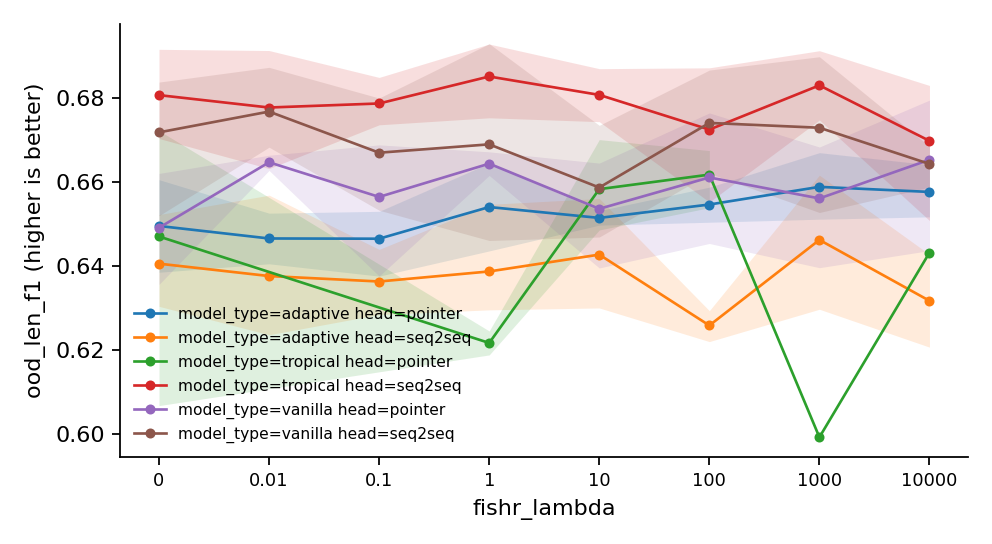
\includegraphics[width=\textwidth]{metric_ood_len_f1.png}
\caption{\texttt{ood\_len\_f1} against \texttt{fishr\_lambda}: the mean over seeds with a 95\% bootstrap CI, one line per combination of the other factors.}
\label{fig:ood_len_f1}
\end{figure}

{\small
\begin{longtable}{lllrlrrr}
\caption{\texttt{ood\_len\_f1} per cell: mean, 95\% bootstrap CI, SD, seeds, diverged runs.}\label{tab:summary-ood_len_f1}\\
\toprule
\texttt{model\_type} & \texttt{head} & \texttt{fishr\_lambda} & mean & 95\% CI & SD & $n$ & div.\\
\midrule
\endhead
adaptive & pointer & 0 & 0.6496 & [0.639, 0.661] & 0.0145 & 5 & 0\\
adaptive & pointer & 0.01 & 0.6466 & [0.641, 0.653] & 0.00783 & 5 & 0\\
adaptive & pointer & 0.1 & 0.6465 & [0.638, 0.653] & 0.00989 & 5 & 0\\
adaptive & pointer & 1 & 0.6541 & [0.644, 0.665] & 0.0135 & 5 & 0\\
adaptive & pointer & 10 & 0.6515 & [0.65, 0.653] & 0.00237 & 5 & 0\\
adaptive & pointer & 100 & 0.6547 & [0.65, 0.659] & 0.00552 & 5 & 0\\
adaptive & pointer & 1000 & 0.6589 & [0.651, 0.667] & 0.0106 & 5 & 0\\
adaptive & pointer & 1e+04 & 0.6577 & [0.652, 0.664] & 0.00796 & 5 & 0\\
adaptive & seq2seq & 0 & 0.6406 & [0.63, 0.652] & 0.014 & 5 & 0\\
adaptive & seq2seq & 0.01 & 0.6376 & [0.624, 0.657] & 0.0216 & 5 & 0\\
adaptive & seq2seq & 0.1 & 0.6363 & [0.628, 0.644] & 0.0105 & 5 & 0\\
adaptive & seq2seq & 1 & 0.6387 & [0.63, 0.655] & 0.0176 & 5 & 0\\
adaptive & seq2seq & 10 & 0.6427 & [0.63, 0.656] & 0.0178 & 5 & 0\\
adaptive & seq2seq & 100 & 0.6259 & [0.622, 0.629] & 0.0049 & 5 & 0\\
adaptive & seq2seq & 1000 & 0.6463 & [0.63, 0.662] & 0.0214 & 5 & 0\\
adaptive & seq2seq & 1e+04 & 0.6317 & [0.621, 0.643] & 0.0141 & 5 & 0\\
tropical & pointer & 0 & 0.6471 & [0.607, 0.672] & 0.0406 & 4 & 0\\
tropical & pointer & 1 & 0.6217 & [0.619, 0.625] & 0.00404 & 2 & 0\\
tropical & pointer & 10 & 0.6584 & [0.649, 0.67] & 0.014 & 5 & 0\\
tropical & pointer & 100 & 0.6618 & [0.654, 0.668] & 0.00706 & 3 & 0\\
tropical & pointer & 1000 & 0.5992 & [--, --] & -- & 1 & 0\\
tropical & pointer & 1e+04 & 0.6432 & [--, --] & -- & 1 & 0\\
tropical & seq2seq & 0 & 0.6808 & [0.67, 0.692] & 0.0143 & 5 & 0\\
tropical & seq2seq & 0.01 & 0.6778 & [0.663, 0.691] & 0.0185 & 5 & 0\\
tropical & seq2seq & 0.1 & 0.6788 & [0.674, 0.685] & 0.00713 & 5 & 0\\
tropical & seq2seq & 1 & 0.6852 & [0.675, 0.693] & 0.0108 & 5 & 0\\
tropical & seq2seq & 10 & 0.6808 & [0.674, 0.687] & 0.00839 & 5 & 0\\
tropical & seq2seq & 100 & 0.6726 & [0.655, 0.687] & 0.0215 & 5 & 0\\
tropical & seq2seq & 1000 & 0.6831 & [0.675, 0.691] & 0.011 & 5 & 0\\
tropical & seq2seq & 1e+04 & 0.6699 & [0.651, 0.683] & 0.0216 & 5 & 0\\
vanilla & pointer & 0 & 0.6491 & [0.636, 0.662] & 0.0173 & 5 & 0\\
vanilla & pointer & 0.01 & 0.6648 & [0.663, 0.666] & 0.00243 & 5 & 0\\
vanilla & pointer & 0.1 & 0.6565 & [0.638, 0.669] & 0.0216 & 5 & 0\\
vanilla & pointer & 1 & 0.6644 & [0.662, 0.667] & 0.00366 & 5 & 0\\
vanilla & pointer & 10 & 0.6537 & [0.64, 0.665] & 0.0167 & 5 & 0\\
vanilla & pointer & 100 & 0.6611 & [0.645, 0.677] & 0.0198 & 5 & 0\\
vanilla & pointer & 1000 & 0.6561 & [0.64, 0.668] & 0.018 & 5 & 0\\
vanilla & pointer & 1e+04 & 0.6654 & [0.644, 0.68] & 0.0243 & 5 & 0\\
vanilla & seq2seq & 0 & 0.6719 & [0.652, 0.684] & 0.0224 & 5 & 0\\
vanilla & seq2seq & 0.01 & 0.6769 & [0.668, 0.687] & 0.0127 & 5 & 0\\
vanilla & seq2seq & 0.1 & 0.667 & [0.653, 0.68] & 0.0173 & 5 & 0\\
vanilla & seq2seq & 1 & 0.669 & [0.646, 0.693] & 0.0299 & 5 & 0\\
vanilla & seq2seq & 10 & 0.6587 & [0.647, 0.674] & 0.0169 & 5 & 0\\
vanilla & seq2seq & 100 & 0.6741 & [0.662, 0.687] & 0.0163 & 5 & 0\\
vanilla & seq2seq & 1000 & 0.673 & [0.653, 0.69] & 0.0237 & 5 & 0\\
vanilla & seq2seq & 1e+04 & 0.6644 & [0.659, 0.669] & 0.00653 & 5 & 0\\
\bottomrule
\end{longtable}
}

{\small
\begin{longtable}{lllrrrl}
\caption{\texttt{ood\_len\_f1}: each level of \texttt{fishr\_lambda} against its control (0), within each combination of the other factors. parametric: Dunnett vs control.}\label{tab:control-ood_len_f1}\\
\toprule
\texttt{model\_type} & \texttt{head} & \texttt{fishr\_lambda} & difference & 95\% CI & $p$ & \\
\midrule
\endhead
adaptive & pointer & 0.01 & -0.002984 & [-0.02, 0.0141] & 0.9962 & \\
adaptive & pointer & 0.1 & -0.003039 & [-0.0201, 0.014] & 0.9958 & \\
adaptive & pointer & 1 & 0.004514 & [-0.0126, 0.0216] & 0.9632 & \\
adaptive & pointer & 10 & 0.00192 & [-0.0151, 0.019] & 0.9998 & \\
adaptive & pointer & 100 & 0.005112 & [-0.012, 0.0222] & 0.9338 & \\
adaptive & pointer & 1000 & 0.009323 & [-0.00774, 0.0264] & 0.5121 & \\
adaptive & pointer & 1e+04 & 0.008116 & [-0.00895, 0.0252] & 0.6491 & \\
adaptive & seq2seq & 0.01 & -0.002953 & [-0.0311, 0.0252] & 0.9999 & \\
adaptive & seq2seq & 0.1 & -0.004254 & [-0.0324, 0.0239] & 0.9985 & \\
adaptive & seq2seq & 1 & -0.001856 & [-0.03, 0.0263] & 1.0000 & \\
adaptive & seq2seq & 10 & 0.002158 & [-0.026, 0.0303] & 1.0000 & \\
adaptive & seq2seq & 100 & -0.01474 & [-0.0429, 0.0135] & 0.5569 & \\
adaptive & seq2seq & 1000 & 0.00567 & [-0.0225, 0.0339] & 0.9915 & \\
adaptive & seq2seq & 1e+04 & -0.008854 & [-0.037, 0.0193] & 0.9184 & \\
tropical & seq2seq & 0.01 & -0.002955 & [-0.0294, 0.0235] & 0.9998 & \\
tropical & seq2seq & 0.1 & -0.001991 & [-0.0284, 0.0245] & 1.0000 & \\
tropical & seq2seq & 1 & 0.004443 & [-0.022, 0.0309] & 0.9970 & \\
tropical & seq2seq & 10 & $5.494\times10^{-5}$ & [-0.0264, 0.0265] & 1.0000 & \\
tropical & seq2seq & 100 & -0.008216 & [-0.0347, 0.0182] & 0.9223 & \\
tropical & seq2seq & 1000 & 0.002329 & [-0.0241, 0.0288] & 1.0000 & \\
tropical & seq2seq & 1e+04 & -0.01091 & [-0.0374, 0.0156] & 0.7703 & \\
vanilla & pointer & 0.01 & 0.01561 & [-0.0145, 0.0457] & 0.5641 & \\
vanilla & pointer & 0.1 & 0.007357 & [-0.0227, 0.0374] & 0.9753 & \\
vanilla & pointer & 1 & 0.01529 & [-0.0148, 0.0454] & 0.5850 & \\
vanilla & pointer & 10 & 0.00452 & [-0.0256, 0.0346] & 0.9985 & \\
vanilla & pointer & 100 & 0.012 & [-0.0181, 0.0421] & 0.7939 & \\
vanilla & pointer & 1000 & 0.007 & [-0.0231, 0.0371] & 0.9809 & \\
vanilla & pointer & 1e+04 & 0.01622 & [-0.0139, 0.0463] & 0.5254 & \\
vanilla & seq2seq & 0.01 & 0.004953 & [-0.0289, 0.0388] & 0.9987 & \\
vanilla & seq2seq & 0.1 & -0.004852 & [-0.0387, 0.029] & 0.9989 & \\
vanilla & seq2seq & 1 & -0.002859 & [-0.0367, 0.031] & 1.0000 & \\
vanilla & seq2seq & 10 & -0.01316 & [-0.047, 0.0207] & 0.8122 & \\
vanilla & seq2seq & 100 & 0.002246 & [-0.0316, 0.0361] & 1.0000 & \\
vanilla & seq2seq & 1000 & 0.001102 & [-0.0328, 0.035] & 1.0000 & \\
vanilla & seq2seq & 1e+04 & -0.007535 & [-0.0414, 0.0264] & 0.9851 & \\
\bottomrule
\end{longtable}
}

{\small
\begin{longtable}{llrrrrr}
\caption{\texttt{ood\_len\_f1} against log10 \texttt{fishr\_lambda}: parametric: OLS slope t-test, seed-bootstrap CI, with the Jonckheere--Terpstra ordered-trend $\tau$ and $p$.}\label{tab:trend-ood_len_f1}\\
\toprule
\texttt{model\_type} & \texttt{head} & estimate & 95\% CI & $p$ & JT $\tau$ & JT $p$\\
\midrule
\endhead
adaptive & pointer & 0.002094 & [0.00146, 0.00307] & 0.0059 & 0.31 & 0.0192\\
adaptive & seq2seq & $-3.834\times10^{-4}$ & [-0.00318, 0.00249] & 0.7842 & -0.0743 & 0.5923\\
tropical & pointer & $-7.584\times10^{-4}$ & [-0.0264, 0.0192] & 0.9051 & 0.115 & 0.7187\\
tropical & seq2seq & $-9.952\times10^{-4}$ & [-0.00306, $5.98\times10^{-4}$] & 0.4339 & -0.0324 & 0.8250\\
vanilla & pointer & $-7.792\times10^{-5}$ & [-0.00103, $7.42\times10^{-4}$] & 0.9558 & 0.00952 & 0.9570\\
vanilla & seq2seq & $-7.303\times10^{-4}$ & [-0.00356, 0.00213] & 0.6412 & -0.0857 & 0.5193\\
\bottomrule
\end{longtable}
}

{\small
\begin{longtable}{lrrrl}
\caption{\texttt{ood\_len\_f1}: paired contrasts by seed, Holm-corrected across the cells. parametric: paired t-test by seed, Holm.}\label{tab:paired-ood_len_f1}\\
\toprule
contrast (within) & difference & 95\% CI & $p$ & \\
\midrule
\endhead
\stackcell{model\_type: tropical - vanilla\\\footnotesize head=pointer fishr\_lambda=0 } & -0.002926 & [-0.0557, 0.0498] & 1.0000 & \\
\stackcell{model\_type: tropical - vanilla\\\footnotesize head=pointer fishr\_lambda=1 } & -0.04397 & [-0.0965, 0.00853] & 0.6561 & \\
\stackcell{model\_type: tropical - vanilla\\\footnotesize head=pointer fishr\_lambda=10 } & 0.004693 & [-0.0125, 0.0219] & 1.0000 & \\
\stackcell{model\_type: tropical - vanilla\\\footnotesize head=pointer fishr\_lambda=100 } & 0.01056 & [-0.0427, 0.0639] & 1.0000 & \\
\stackcell{model\_type: tropical - vanilla\\\footnotesize head=seq2seq fishr\_lambda=0 } & 0.008877 & [-0.0175, 0.0352] & 1.0000 & \\
\stackcell{model\_type: tropical - vanilla\\\footnotesize head=seq2seq fishr\_lambda=0.01 } & $9.691\times10^{-4}$ & [-0.0236, 0.0255] & 1.0000 & \\
\stackcell{model\_type: tropical - vanilla\\\footnotesize head=seq2seq fishr\_lambda=0.1 } & 0.01174 & [-0.00557, 0.029] & 1.0000 & \\
\stackcell{model\_type: tropical - vanilla\\\footnotesize head=seq2seq fishr\_lambda=1 } & 0.01618 & [-0.0117, 0.0441] & 1.0000 & \\
\stackcell{model\_type: tropical - vanilla\\\footnotesize head=seq2seq fishr\_lambda=10 } & 0.02209 & [0.00673, 0.0374] & 0.1946 & \\
\stackcell{model\_type: tropical - vanilla\\\footnotesize head=seq2seq fishr\_lambda=100 } & -0.001585 & [-0.0412, 0.038] & 1.0000 & \\
\stackcell{model\_type: tropical - vanilla\\\footnotesize head=seq2seq fishr\_lambda=1000 } & 0.0101 & [-0.0254, 0.0456] & 1.0000 & \\
\stackcell{model\_type: tropical - vanilla\\\footnotesize head=seq2seq fishr\_lambda=1e+04 } & 0.005507 & [-0.0222, 0.0332] & 1.0000 & \\
\stackcell{model\_type: adaptive - vanilla\\\footnotesize head=pointer fishr\_lambda=0 } & $4.302\times10^{-4}$ & [-0.0328, 0.0337] & 1.0000 & \\
\stackcell{model\_type: adaptive - vanilla\\\footnotesize head=pointer fishr\_lambda=0.01 } & -0.01817 & [-0.0261, -0.0102] & 0.0477 & *\\
\stackcell{model\_type: adaptive - vanilla\\\footnotesize head=pointer fishr\_lambda=0.1 } & -0.009965 & [-0.0422, 0.0222] & 1.0000 & \\
\stackcell{model\_type: adaptive - vanilla\\\footnotesize head=pointer fishr\_lambda=1 } & -0.01034 & [-0.0291, 0.00841] & 1.0000 & \\
\stackcell{model\_type: adaptive - vanilla\\\footnotesize head=pointer fishr\_lambda=10 } & -0.002169 & [-0.0233, 0.019] & 1.0000 & \\
\stackcell{model\_type: adaptive - vanilla\\\footnotesize head=pointer fishr\_lambda=100 } & -0.006454 & [-0.0298, 0.0169] & 1.0000 & \\
\stackcell{model\_type: adaptive - vanilla\\\footnotesize head=pointer fishr\_lambda=1000 } & 0.002754 & [-0.0245, 0.03] & 1.0000 & \\
\stackcell{model\_type: adaptive - vanilla\\\footnotesize head=pointer fishr\_lambda=1e+04 } & -0.007674 & [-0.035, 0.0197] & 1.0000 & \\
\stackcell{model\_type: adaptive - vanilla\\\footnotesize head=seq2seq fishr\_lambda=0 } & -0.03131 & [-0.0596, -0.00301] & 0.4469 & \\
\stackcell{model\_type: adaptive - vanilla\\\footnotesize head=seq2seq fishr\_lambda=0.01 } & -0.03922 & [-0.0778, $-6.39\times10^{-4}$] & 0.5248 & \\
\stackcell{model\_type: adaptive - vanilla\\\footnotesize head=seq2seq fishr\_lambda=0.1 } & -0.03071 & [-0.0457, -0.0157] & 0.0657 & \\
\stackcell{model\_type: adaptive - vanilla\\\footnotesize head=seq2seq fishr\_lambda=1 } & -0.03031 & [-0.0861, 0.0254] & 1.0000 & \\
\stackcell{model\_type: adaptive - vanilla\\\footnotesize head=seq2seq fishr\_lambda=10 } & -0.01599 & [-0.0434, 0.0114] & 1.0000 & \\
\stackcell{model\_type: adaptive - vanilla\\\footnotesize head=seq2seq fishr\_lambda=100 } & -0.04829 & [-0.0674, -0.0292] & 0.0348 & *\\
\stackcell{model\_type: adaptive - vanilla\\\footnotesize head=seq2seq fishr\_lambda=1000 } & -0.02674 & [-0.0619, 0.00839] & 1.0000 & \\
\stackcell{model\_type: adaptive - vanilla\\\footnotesize head=seq2seq fishr\_lambda=1e+04 } & -0.03263 & [-0.0571, -0.00821] & 0.2686 & \\
\stackcell{head: pointer - seq2seq\\\footnotesize model\_type=adaptive fishr\_lambda=0 } & 0.008989 & [-0.0192, 0.0372] & 1.0000 & \\
\stackcell{head: pointer - seq2seq\\\footnotesize model\_type=adaptive fishr\_lambda=0.01 } & 0.008958 & [-0.0163, 0.0342] & 1.0000 & \\
\stackcell{head: pointer - seq2seq\\\footnotesize model\_type=adaptive fishr\_lambda=0.1 } & 0.0102 & [-0.0124, 0.0328] & 1.0000 & \\
\stackcell{head: pointer - seq2seq\\\footnotesize model\_type=adaptive fishr\_lambda=1 } & 0.01536 & [-0.0208, 0.0515] & 1.0000 & \\
\stackcell{head: pointer - seq2seq\\\footnotesize model\_type=adaptive fishr\_lambda=10 } & 0.008752 & [-0.0133, 0.0308] & 1.0000 & \\
\stackcell{head: pointer - seq2seq\\\footnotesize model\_type=adaptive fishr\_lambda=100 } & 0.02884 & [0.02, 0.0376] & 0.0162 & *\\
\stackcell{head: pointer - seq2seq\\\footnotesize model\_type=adaptive fishr\_lambda=1000 } & 0.01264 & [-0.0123, 0.0376] & 1.0000 & \\
\stackcell{head: pointer - seq2seq\\\footnotesize model\_type=adaptive fishr\_lambda=1e+04 } & 0.02596 & [0.0165, 0.0354] & 0.0301 & *\\
\stackcell{head: pointer - seq2seq\\\footnotesize model\_type=tropical fishr\_lambda=0 } & -0.03676 & [-0.123, 0.0497] & 1.0000 & \\
\stackcell{head: pointer - seq2seq\\\footnotesize model\_type=tropical fishr\_lambda=1 } & -0.05749 & [-0.225, 0.11] & 1.0000 & \\
\stackcell{head: pointer - seq2seq\\\footnotesize model\_type=tropical fishr\_lambda=10 } & -0.02247 & [-0.0412, -0.00372] & 0.5119 & \\
\stackcell{head: pointer - seq2seq\\\footnotesize model\_type=tropical fishr\_lambda=100 } & -0.02182 & [-0.038, -0.00564] & 0.5119 & \\
\stackcell{head: pointer - seq2seq\\\footnotesize model\_type=vanilla fishr\_lambda=0 } & -0.02275 & [-0.0511, 0.0056] & 1.0000 & \\
\stackcell{head: pointer - seq2seq\\\footnotesize model\_type=vanilla fishr\_lambda=0.01 } & -0.01209 & [-0.028, 0.0038] & 1.0000 & \\
\stackcell{head: pointer - seq2seq\\\footnotesize model\_type=vanilla fishr\_lambda=0.1 } & -0.01054 & [-0.047, 0.0259] & 1.0000 & \\
\stackcell{head: pointer - seq2seq\\\footnotesize model\_type=vanilla fishr\_lambda=1 } & -0.004605 & [-0.0405, 0.0313] & 1.0000 & \\
\stackcell{head: pointer - seq2seq\\\footnotesize model\_type=vanilla fishr\_lambda=10 } & -0.005074 & [-0.0333, 0.0232] & 1.0000 & \\
\stackcell{head: pointer - seq2seq\\\footnotesize model\_type=vanilla fishr\_lambda=100 } & -0.013 & [-0.0444, 0.0184] & 1.0000 & \\
\stackcell{head: pointer - seq2seq\\\footnotesize model\_type=vanilla fishr\_lambda=1000 } & -0.01685 & [-0.0383, 0.00461] & 1.0000 & \\
\stackcell{head: pointer - seq2seq\\\footnotesize model\_type=vanilla fishr\_lambda=1e+04 } & 0.001003 & [-0.0333, 0.0353] & 1.0000 & \\
\bottomrule
\end{longtable}
}

\clearpage
\appendix
\section{Other metrics}
\subsection{\texttt{ood\_len\_exact}}
\begin{figure}[tbp]
\centering
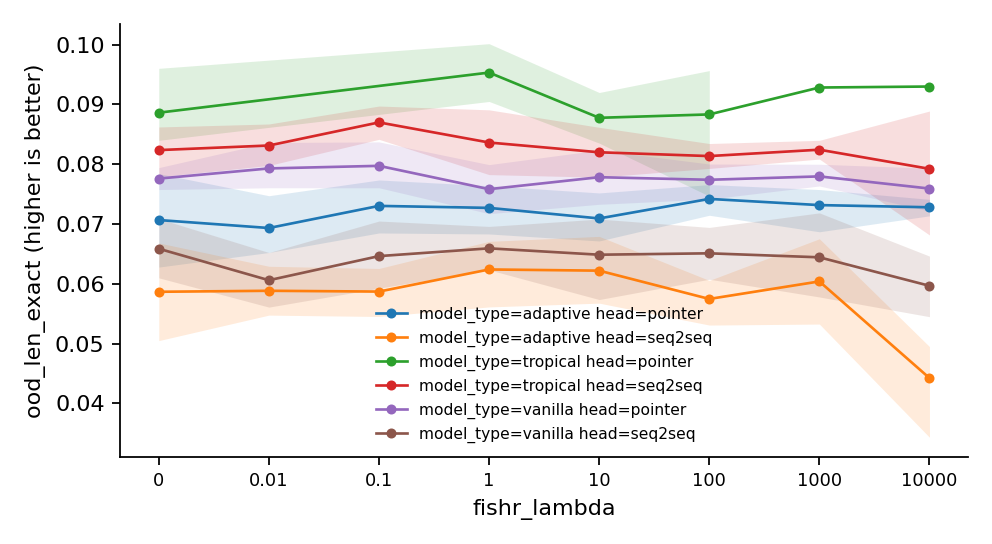
\includegraphics[width=\textwidth]{metric_ood_len_exact.png}
\caption{\texttt{ood\_len\_exact} against \texttt{fishr\_lambda}: the mean over seeds with a 95\% bootstrap CI, one line per combination of the other factors.}
\label{fig:ood_len_exact}
\end{figure}

{\small
\begin{longtable}{lllrlrrr}
\caption{\texttt{ood\_len\_exact} per cell: mean, 95\% bootstrap CI, SD, seeds, diverged runs.}\label{tab:summary-ood_len_exact}\\
\toprule
\texttt{model\_type} & \texttt{head} & \texttt{fishr\_lambda} & mean & 95\% CI & SD & $n$ & div.\\
\midrule
\endhead
adaptive & pointer & 0 & 0.07067 & [0.0628, 0.0784] & 0.0103 & 5 & 0\\
adaptive & pointer & 0.01 & 0.06933 & [0.0652, 0.0747] & 0.00615 & 5 & 0\\
adaptive & pointer & 0.1 & 0.07303 & [0.0685, 0.0774] & 0.00544 & 5 & 0\\
adaptive & pointer & 1 & 0.0727 & [0.0683, 0.0764] & 0.00542 & 5 & 0\\
adaptive & pointer & 10 & 0.07093 & [0.0672, 0.0752] & 0.00505 & 5 & 0\\
adaptive & pointer & 100 & 0.0742 & [0.0715, 0.0766] & 0.00332 & 5 & 0\\
adaptive & pointer & 1000 & 0.07317 & [0.0687, 0.0758] & 0.00474 & 5 & 0\\
adaptive & pointer & 1e+04 & 0.0728 & [0.0714, 0.0741] & 0.0018 & 5 & 0\\
adaptive & seq2seq & 0 & 0.05867 & [0.0505, 0.0668] & 0.0107 & 5 & 0\\
adaptive & seq2seq & 0.01 & 0.05883 & [0.0548, 0.0629] & 0.00536 & 5 & 0\\
adaptive & seq2seq & 0.1 & 0.0587 & [0.0545, 0.0626] & 0.00514 & 5 & 0\\
adaptive & seq2seq & 1 & 0.0624 & [0.0561, 0.0671] & 0.00716 & 5 & 0\\
adaptive & seq2seq & 10 & 0.0622 & [0.0568, 0.0679] & 0.00728 & 5 & 0\\
adaptive & seq2seq & 100 & 0.05747 & [0.0531, 0.0606] & 0.00502 & 5 & 0\\
adaptive & seq2seq & 1000 & 0.0604 & [0.0533, 0.0675] & 0.00938 & 5 & 0\\
adaptive & seq2seq & 1e+04 & 0.04423 & [0.0343, 0.0495] & 0.011 & 5 & 0\\
tropical & pointer & 0 & 0.08862 & [0.084, 0.096] & 0.00768 & 4 & 0\\
tropical & pointer & 1 & 0.09533 & [0.0905, 0.1] & 0.00684 & 2 & 0\\
tropical & pointer & 10 & 0.08777 & [0.0835, 0.092] & 0.00536 & 5 & 0\\
tropical & pointer & 100 & 0.08833 & [0.0747, 0.0957] & 0.0118 & 3 & 0\\
tropical & pointer & 1000 & 0.09283 & [--, --] & -- & 1 & 0\\
tropical & pointer & 1e+04 & 0.093 & [--, --] & -- & 1 & 0\\
tropical & seq2seq & 0 & 0.08237 & [0.0779, 0.0862] & 0.00505 & 5 & 0\\
tropical & seq2seq & 0.01 & 0.08313 & [0.0798, 0.0867] & 0.00455 & 5 & 0\\
tropical & seq2seq & 0.1 & 0.087 & [0.0842, 0.0897] & 0.00345 & 5 & 0\\
tropical & seq2seq & 1 & 0.08363 & [0.0783, 0.0891] & 0.00704 & 5 & 0\\
tropical & seq2seq & 10 & 0.082 & [0.0778, 0.0862] & 0.00569 & 5 & 0\\
tropical & seq2seq & 100 & 0.08137 & [0.0793, 0.0835] & 0.00269 & 5 & 0\\
tropical & seq2seq & 1000 & 0.08243 & [0.0809, 0.084] & 0.00211 & 5 & 0\\
tropical & seq2seq & 1e+04 & 0.07923 & [0.0682, 0.0889] & 0.0129 & 5 & 0\\
vanilla & pointer & 0 & 0.0776 & [0.0758, 0.0794] & 0.00243 & 5 & 0\\
vanilla & pointer & 0.01 & 0.0793 & [0.0761, 0.0836] & 0.00489 & 5 & 0\\
vanilla & pointer & 0.1 & 0.07973 & [0.0761, 0.0837] & 0.00497 & 5 & 0\\
vanilla & pointer & 1 & 0.07583 & [0.0717, 0.0799] & 0.00548 & 5 & 0\\
vanilla & pointer & 10 & 0.07783 & [0.0733, 0.0824] & 0.00598 & 5 & 0\\
vanilla & pointer & 100 & 0.0774 & [0.0742, 0.08] & 0.00394 & 5 & 0\\
vanilla & pointer & 1000 & 0.07797 & [0.0764, 0.08] & 0.0022 & 5 & 0\\
vanilla & pointer & 1e+04 & 0.07593 & [0.0722, 0.0793] & 0.00462 & 5 & 0\\
vanilla & seq2seq & 0 & 0.06587 & [0.061, 0.0709] & 0.00641 & 5 & 0\\
vanilla & seq2seq & 0.01 & 0.0606 & [0.0561, 0.0652] & 0.00545 & 5 & 0\\
vanilla & seq2seq & 0.1 & 0.06463 & [0.0593, 0.0705] & 0.00713 & 5 & 0\\
vanilla & seq2seq & 1 & 0.06593 & [0.0623, 0.0696] & 0.00493 & 5 & 0\\
vanilla & seq2seq & 10 & 0.06487 & [0.0574, 0.0708] & 0.00908 & 5 & 0\\
vanilla & seq2seq & 100 & 0.0651 & [0.0608, 0.0694] & 0.00566 & 5 & 0\\
vanilla & seq2seq & 1000 & 0.06443 & [0.0578, 0.0719] & 0.00891 & 5 & 0\\
vanilla & seq2seq & 1e+04 & 0.05967 & [0.0545, 0.0646] & 0.00649 & 5 & 0\\
\bottomrule
\end{longtable}
}

{\small
\begin{longtable}{lllrrrl}
\caption{\texttt{ood\_len\_exact}: each level of \texttt{fishr\_lambda} against its control (0), within each combination of the other factors. parametric: Dunnett vs control.}\label{tab:control-ood_len_exact}\\
\toprule
\texttt{model\_type} & \texttt{head} & \texttt{fishr\_lambda} & difference & 95\% CI & $p$ & \\
\midrule
\endhead
adaptive & pointer & 0.01 & -0.001333 & [-0.0114, 0.00872] & 0.9993 & \\
adaptive & pointer & 0.1 & 0.002367 & [-0.00769, 0.0124] & 0.9798 & \\
adaptive & pointer & 1 & 0.002033 & [-0.00802, 0.0121] & 0.9912 & \\
adaptive & pointer & 10 & $2.667\times10^{-4}$ & [-0.00979, 0.0103] & 1.0000 & \\
adaptive & pointer & 100 & 0.003533 & [-0.00652, 0.0136] & 0.8702 & \\
adaptive & pointer & 1000 & 0.0025 & [-0.00756, 0.0126] & 0.9731 & \\
adaptive & pointer & 1e+04 & 0.002133 & [-0.00792, 0.0122] & 0.9885 & \\
adaptive & seq2seq & 0.01 & $1.667\times10^{-4}$ & [-0.0137, 0.0141] & 1.0000 & \\
adaptive & seq2seq & 0.1 & $3.333\times10^{-5}$ & [-0.0139, 0.0139] & 1.0000 & \\
adaptive & seq2seq & 1 & 0.003733 & [-0.0102, 0.0176] & 0.9603 & \\
adaptive & seq2seq & 10 & 0.003533 & [-0.0104, 0.0174] & 0.9698 & \\
adaptive & seq2seq & 100 & -0.0012 & [-0.0151, 0.0127] & 1.0000 & \\
adaptive & seq2seq & 1000 & 0.001733 & [-0.0122, 0.0156] & 0.9995 & \\
adaptive & seq2seq & 1e+04 & -0.01443 & [-0.0283, $-5.38\times10^{-4}$] & 0.0392 & *\\
tropical & seq2seq & 0.01 & $7.667\times10^{-4}$ & [-0.0102, 0.0118] & 1.0000 & \\
tropical & seq2seq & 0.1 & 0.004633 & [-0.00638, 0.0156] & 0.7543 & \\
tropical & seq2seq & 1 & 0.001267 & [-0.00974, 0.0123] & 0.9997 & \\
tropical & seq2seq & 10 & $-3.667\times10^{-4}$ & [-0.0114, 0.0106] & 1.0000 & \\
tropical & seq2seq & 100 & -0.001 & [-0.012, 0.01] & 0.9999 & \\
tropical & seq2seq & 1000 & $6.667\times10^{-5}$ & [-0.0109, 0.0111] & 1.0000 & \\
tropical & seq2seq & 1e+04 & -0.003133 & [-0.0141, 0.00788] & 0.9477 & \\
vanilla & pointer & 0.01 & 0.0017 & [-0.00616, 0.00956] & 0.9872 & \\
vanilla & pointer & 0.1 & 0.002133 & [-0.00573, 0.00999] & 0.9583 & \\
vanilla & pointer & 1 & -0.001767 & [-0.00963, 0.00609] & 0.9842 & \\
vanilla & pointer & 10 & $2.333\times10^{-4}$ & [-0.00763, 0.00809] & 1.0000 & \\
vanilla & pointer & 100 & $-2.000\times10^{-4}$ & [-0.00806, 0.00766] & 1.0000 & \\
vanilla & pointer & 1000 & $3.667\times10^{-4}$ & [-0.00749, 0.00823] & 1.0000 & \\
vanilla & pointer & 1e+04 & -0.001667 & [-0.00953, 0.00619] & 0.9885 & \\
vanilla & seq2seq & 0.01 & -0.005267 & [-0.0173, 0.0068] & 0.7249 & \\
vanilla & seq2seq & 0.1 & -0.001233 & [-0.0133, 0.0108] & 0.9999 & \\
vanilla & seq2seq & 1 & $6.667\times10^{-5}$ & [-0.012, 0.0121] & 1.0000 & \\
vanilla & seq2seq & 10 & -0.001 & [-0.0131, 0.0111] & 1.0000 & \\
vanilla & seq2seq & 100 & $-7.667\times10^{-4}$ & [-0.0128, 0.0113] & 1.0000 & \\
vanilla & seq2seq & 1000 & -0.001433 & [-0.0135, 0.0106] & 0.9997 & \\
vanilla & seq2seq & 1e+04 & -0.0062 & [-0.0183, 0.00587] & 0.5743 & \\
\bottomrule
\end{longtable}
}

{\small
\begin{longtable}{llrrrrr}
\caption{\texttt{ood\_len\_exact} against log10 \texttt{fishr\_lambda}: parametric: OLS slope t-test, seed-bootstrap CI, with the Jonckheere--Terpstra ordered-trend $\tau$ and $p$.}\label{tab:trend-ood_len_exact}\\
\toprule
\texttt{model\_type} & \texttt{head} & estimate & 95\% CI & $p$ & JT $\tau$ & JT $p$\\
\midrule
\endhead
adaptive & pointer & $4.345\times10^{-4}$ & [$-2.75\times10^{-4}$, 0.0012] & 0.2688 & 0.118 & 0.3683\\
adaptive & seq2seq & -0.001619 & [-0.00256, $-6.77\times10^{-4}$] & 0.0305 & -0.23 & 0.0760\\
tropical & pointer & $-7.778\times10^{-5}$ & [-0.00167, 0.00434] & 0.9684 & -0.0385 & 0.9424\\
tropical & seq2seq & $-8.250\times10^{-4}$ & [-0.00145, $-3.81\times10^{-4}$] & 0.1213 & -0.179 & 0.1808\\
vanilla & pointer & $-4.310\times10^{-4}$ & [-0.00101, $6.90\times10^{-5}$] & 0.2643 & -0.12 & 0.3837\\
vanilla & seq2seq & $-1.440\times10^{-4}$ & [$-9.94\times10^{-4}$, $5.20\times10^{-4}$] & 0.8044 & -0.0286 & 0.8344\\
\bottomrule
\end{longtable}
}

{\small
\begin{longtable}{lrrrl}
\caption{\texttt{ood\_len\_exact}: paired contrasts by seed, Holm-corrected across the cells. parametric: paired t-test by seed, Holm.}\label{tab:paired-ood_len_exact}\\
\toprule
contrast (within) & difference & 95\% CI & $p$ & \\
\midrule
\endhead
\stackcell{model\_type: tropical - vanilla\\\footnotesize head=pointer fishr\_lambda=0 } & 0.01171 & [0.00296, 0.0205] & 0.0995 & \\
\stackcell{model\_type: tropical - vanilla\\\footnotesize head=pointer fishr\_lambda=1 } & 0.02483 & [-0.0599, 0.11] & 0.3339 & \\
\stackcell{model\_type: tropical - vanilla\\\footnotesize head=pointer fishr\_lambda=10 } & 0.009933 & [$-7.34\times10^{-4}$, 0.0206] & 0.1830 & \\
\stackcell{model\_type: tropical - vanilla\\\footnotesize head=pointer fishr\_lambda=100 } & 0.01211 & [-0.0203, 0.0445] & 0.3339 & \\
\stackcell{model\_type: tropical - vanilla\\\footnotesize head=seq2seq fishr\_lambda=0 } & 0.0165 & [0.0116, 0.0214] & 0.0078 & *\\
\stackcell{model\_type: tropical - vanilla\\\footnotesize head=seq2seq fishr\_lambda=0.01 } & 0.02253 & [0.0135, 0.0316] & 0.0232 & *\\
\stackcell{model\_type: tropical - vanilla\\\footnotesize head=seq2seq fishr\_lambda=0.1 } & 0.02237 & [0.0167, 0.0281] & 0.0048 & *\\
\stackcell{model\_type: tropical - vanilla\\\footnotesize head=seq2seq fishr\_lambda=1 } & 0.0177 & [0.00628, 0.0291] & 0.0756 & \\
\stackcell{model\_type: tropical - vanilla\\\footnotesize head=seq2seq fishr\_lambda=10 } & 0.01713 & [0.0102, 0.0241] & 0.0232 & *\\
\stackcell{model\_type: tropical - vanilla\\\footnotesize head=seq2seq fishr\_lambda=100 } & 0.01627 & [0.00889, 0.0236] & 0.0289 & *\\
\stackcell{model\_type: tropical - vanilla\\\footnotesize head=seq2seq fishr\_lambda=1000 } & 0.018 & [0.00879, 0.0272] & 0.0391 & *\\
\stackcell{model\_type: tropical - vanilla\\\footnotesize head=seq2seq fishr\_lambda=1e+04 } & 0.01957 & [0.00509, 0.034] & 0.0995 & \\
\stackcell{model\_type: adaptive - vanilla\\\footnotesize head=pointer fishr\_lambda=0 } & -0.006933 & [-0.0173, 0.00339] & 1.0000 & \\
\stackcell{model\_type: adaptive - vanilla\\\footnotesize head=pointer fishr\_lambda=0.01 } & -0.009967 & [-0.0187, -0.00124] & 0.5080 & \\
\stackcell{model\_type: adaptive - vanilla\\\footnotesize head=pointer fishr\_lambda=0.1 } & -0.0067 & [-0.00998, -0.00342] & 0.0760 & \\
\stackcell{model\_type: adaptive - vanilla\\\footnotesize head=pointer fishr\_lambda=1 } & -0.003133 & [-0.0135, 0.00724] & 1.0000 & \\
\stackcell{model\_type: adaptive - vanilla\\\footnotesize head=pointer fishr\_lambda=10 } & -0.0069 & [-0.0132, $-6.36\times10^{-4}$] & 0.5281 & \\
\stackcell{model\_type: adaptive - vanilla\\\footnotesize head=pointer fishr\_lambda=100 } & -0.0032 & [-0.00724, $8.40\times10^{-4}$] & 1.0000 & \\
\stackcell{model\_type: adaptive - vanilla\\\footnotesize head=pointer fishr\_lambda=1000 } & -0.0048 & [-0.012, 0.00237] & 1.0000 & \\
\stackcell{model\_type: adaptive - vanilla\\\footnotesize head=pointer fishr\_lambda=1e+04 } & -0.003133 & [-0.00972, 0.00346] & 1.0000 & \\
\stackcell{model\_type: adaptive - vanilla\\\footnotesize head=seq2seq fishr\_lambda=0 } & -0.0072 & [-0.0227, 0.00833] & 1.0000 & \\
\stackcell{model\_type: adaptive - vanilla\\\footnotesize head=seq2seq fishr\_lambda=0.01 } & -0.001767 & [-0.00842, 0.00489] & 1.0000 & \\
\stackcell{model\_type: adaptive - vanilla\\\footnotesize head=seq2seq fishr\_lambda=0.1 } & -0.005933 & [-0.0148, 0.00291] & 1.0000 & \\
\stackcell{model\_type: adaptive - vanilla\\\footnotesize head=seq2seq fishr\_lambda=1 } & -0.003533 & [-0.0115, 0.00446] & 1.0000 & \\
\stackcell{model\_type: adaptive - vanilla\\\footnotesize head=seq2seq fishr\_lambda=10 } & -0.002667 & [-0.0115, 0.00612] & 1.0000 & \\
\stackcell{model\_type: adaptive - vanilla\\\footnotesize head=seq2seq fishr\_lambda=100 } & -0.007633 & [-0.0166, 0.00134] & 1.0000 & \\
\stackcell{model\_type: adaptive - vanilla\\\footnotesize head=seq2seq fishr\_lambda=1000 } & -0.004033 & [-0.0209, 0.0128] & 1.0000 & \\
\stackcell{model\_type: adaptive - vanilla\\\footnotesize head=seq2seq fishr\_lambda=1e+04 } & -0.01543 & [-0.0351, 0.00422] & 1.0000 & \\
\stackcell{head: pointer - seq2seq\\\footnotesize model\_type=adaptive fishr\_lambda=0 } & 0.012 & [-0.00818, 0.0322] & 0.4278 & \\
\stackcell{head: pointer - seq2seq\\\footnotesize model\_type=adaptive fishr\_lambda=0.01 } & 0.0105 & [-0.00105, 0.0221] & 0.4278 & \\
\stackcell{head: pointer - seq2seq\\\footnotesize model\_type=adaptive fishr\_lambda=0.1 } & 0.01433 & [0.00415, 0.0245] & 0.2443 & \\
\stackcell{head: pointer - seq2seq\\\footnotesize model\_type=adaptive fishr\_lambda=1 } & 0.0103 & [$2.09\times10^{-4}$, 0.0204] & 0.4244 & \\
\stackcell{head: pointer - seq2seq\\\footnotesize model\_type=adaptive fishr\_lambda=10 } & 0.008733 & [-0.00212, 0.0196] & 0.4278 & \\
\stackcell{head: pointer - seq2seq\\\footnotesize model\_type=adaptive fishr\_lambda=100 } & 0.01673 & [0.00839, 0.0251] & 0.0866 & \\
\stackcell{head: pointer - seq2seq\\\footnotesize model\_type=adaptive fishr\_lambda=1000 } & 0.01277 & [0.00362, 0.0219] & 0.2443 & \\
\stackcell{head: pointer - seq2seq\\\footnotesize model\_type=adaptive fishr\_lambda=1e+04 } & 0.02857 & [0.0168, 0.0403] & 0.0481 & *\\
\stackcell{head: pointer - seq2seq\\\footnotesize model\_type=tropical fishr\_lambda=0 } & 0.007333 & [0.00104, 0.0136] & 0.3404 & \\
\stackcell{head: pointer - seq2seq\\\footnotesize model\_type=tropical fishr\_lambda=1 } & 0.017 & [-0.00629, 0.0403] & 0.4278 & \\
\stackcell{head: pointer - seq2seq\\\footnotesize model\_type=tropical fishr\_lambda=10 } & 0.005767 & [-0.00131, 0.0128] & 0.4278 & \\
\stackcell{head: pointer - seq2seq\\\footnotesize model\_type=tropical fishr\_lambda=100 } & 0.006833 & [-0.0219, 0.0356] & 0.4278 & \\
\stackcell{head: pointer - seq2seq\\\footnotesize model\_type=vanilla fishr\_lambda=0 } & 0.01173 & [0.00671, 0.0168] & 0.0523 & \\
\stackcell{head: pointer - seq2seq\\\footnotesize model\_type=vanilla fishr\_lambda=0.01 } & 0.0187 & [0.00759, 0.0298] & 0.1422 & \\
\stackcell{head: pointer - seq2seq\\\footnotesize model\_type=vanilla fishr\_lambda=0.1 } & 0.0151 & [0.0072, 0.023] & 0.0970 & \\
\stackcell{head: pointer - seq2seq\\\footnotesize model\_type=vanilla fishr\_lambda=1 } & 0.0099 & [$-2.39\times10^{-4}$, 0.02] & 0.4278 & \\
\stackcell{head: pointer - seq2seq\\\footnotesize model\_type=vanilla fishr\_lambda=10 } & 0.01297 & [$-8.11\times10^{-4}$, 0.0267] & 0.4278 & \\
\stackcell{head: pointer - seq2seq\\\footnotesize model\_type=vanilla fishr\_lambda=100 } & 0.0123 & [0.00308, 0.0215] & 0.2492 & \\
\stackcell{head: pointer - seq2seq\\\footnotesize model\_type=vanilla fishr\_lambda=1000 } & 0.01353 & [0.0027, 0.0244] & 0.2815 & \\
\stackcell{head: pointer - seq2seq\\\footnotesize model\_type=vanilla fishr\_lambda=1e+04 } & 0.01627 & [0.0127, 0.0199] & 0.0047 & *\\
\bottomrule
\end{longtable}
}

\subsection{\texttt{ood\_val\_f1}}
\begin{figure}[tbp]
\centering
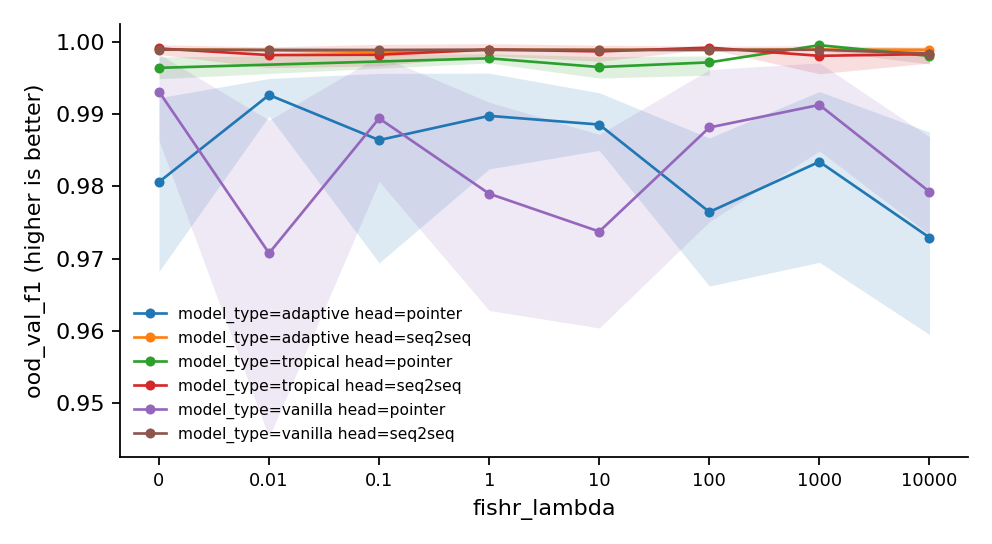
\includegraphics[width=\textwidth]{metric_ood_val_f1.png}
\caption{\texttt{ood\_val\_f1} against \texttt{fishr\_lambda}: the mean over seeds with a 95\% bootstrap CI, one line per combination of the other factors.}
\label{fig:ood_val_f1}
\end{figure}

{\small
\begin{longtable}{lllrlrrr}
\caption{\texttt{ood\_val\_f1} per cell: mean, 95\% bootstrap CI, SD, seeds, diverged runs.}\label{tab:summary-ood_val_f1}\\
\toprule
\texttt{model\_type} & \texttt{head} & \texttt{fishr\_lambda} & mean & 95\% CI & SD & $n$ & div.\\
\midrule
\endhead
adaptive & pointer & 0 & 0.9806 & [0.968, 0.992] & 0.0149 & 5 & 0\\
adaptive & pointer & 0.01 & 0.9927 & [0.99, 0.995] & 0.0035 & 5 & 0\\
adaptive & pointer & 0.1 & 0.9864 & [0.969, 0.996] & 0.0187 & 5 & 0\\
adaptive & pointer & 1 & 0.9898 & [0.982, 0.996] & 0.00874 & 5 & 0\\
adaptive & pointer & 10 & 0.9886 & [0.985, 0.993] & 0.00539 & 5 & 0\\
adaptive & pointer & 100 & 0.9765 & [0.966, 0.987] & 0.0136 & 5 & 0\\
adaptive & pointer & 1000 & 0.9834 & [0.969, 0.993] & 0.0159 & 5 & 0\\
adaptive & pointer & 1e+04 & 0.9729 & [0.96, 0.988] & 0.0185 & 5 & 0\\
adaptive & seq2seq & 0 & 0.999 & [0.999, 0.999] & $2.32\times10^{-4}$ & 5 & 0\\
adaptive & seq2seq & 0.01 & 0.9989 & [0.999, 0.999] & $8.08\times10^{-5}$ & 5 & 0\\
adaptive & seq2seq & 0.1 & 0.9986 & [0.998, 0.999] & $7.15\times10^{-4}$ & 5 & 0\\
adaptive & seq2seq & 1 & 0.9989 & [0.999, 0.999] & $1.21\times10^{-4}$ & 5 & 0\\
adaptive & seq2seq & 10 & 0.9989 & [0.999, 0.999] & $1.36\times10^{-4}$ & 5 & 0\\
adaptive & seq2seq & 100 & 0.9989 & [0.999, 0.999] & $1.37\times10^{-4}$ & 5 & 0\\
adaptive & seq2seq & 1000 & 0.999 & [0.999, 0.999] & $2.39\times10^{-4}$ & 5 & 0\\
adaptive & seq2seq & 1e+04 & 0.9989 & [0.999, 0.999] & $1.31\times10^{-4}$ & 5 & 0\\
tropical & pointer & 0 & 0.9964 & [0.995, 0.998] & 0.00177 & 4 & 0\\
tropical & pointer & 1 & 0.9977 & [0.997, 0.998] & $9.08\times10^{-4}$ & 2 & 0\\
tropical & pointer & 10 & 0.9965 & [0.995, 0.998] & 0.00197 & 5 & 0\\
tropical & pointer & 100 & 0.9972 & [0.995, 0.998] & 0.00153 & 3 & 0\\
tropical & pointer & 1000 & 0.9996 & [--, --] & -- & 1 & 0\\
tropical & pointer & 1e+04 & 0.9981 & [--, --] & -- & 1 & 0\\
tropical & seq2seq & 0 & 0.9991 & [0.998, 1] & $9.24\times10^{-4}$ & 5 & 0\\
tropical & seq2seq & 0.01 & 0.9982 & [0.996, 0.999] & 0.00191 & 5 & 0\\
tropical & seq2seq & 0.1 & 0.9982 & [0.997, 1] & 0.00188 & 5 & 0\\
tropical & seq2seq & 1 & 0.9989 & [0.998, 1] & 0.00106 & 5 & 0\\
tropical & seq2seq & 10 & 0.9987 & [0.997, 1] & 0.00155 & 5 & 0\\
tropical & seq2seq & 100 & 0.9992 & [0.999, 0.999] & $2.39\times10^{-4}$ & 5 & 0\\
tropical & seq2seq & 1000 & 0.9981 & [0.996, 0.999] & 0.00278 & 5 & 0\\
tropical & seq2seq & 1e+04 & 0.9983 & [0.997, 0.999] & 0.00141 & 5 & 0\\
vanilla & pointer & 0 & 0.9931 & [0.986, 0.998] & 0.00765 & 5 & 0\\
vanilla & pointer & 0.01 & 0.9708 & [0.945, 0.989] & 0.0287 & 5 & 0\\
vanilla & pointer & 0.1 & 0.9894 & [0.981, 0.998] & 0.0117 & 5 & 0\\
vanilla & pointer & 1 & 0.979 & [0.963, 0.992] & 0.0186 & 5 & 0\\
vanilla & pointer & 10 & 0.9738 & [0.96, 0.987] & 0.0177 & 5 & 0\\
vanilla & pointer & 100 & 0.9882 & [0.975, 0.996] & 0.0148 & 5 & 0\\
vanilla & pointer & 1000 & 0.9913 & [0.985, 0.997] & 0.00811 & 5 & 0\\
vanilla & pointer & 1e+04 & 0.9793 & [0.973, 0.987] & 0.00927 & 5 & 0\\
vanilla & seq2seq & 0 & 0.9989 & [0.999, 0.999] & $1.50\times10^{-4}$ & 5 & 0\\
vanilla & seq2seq & 0.01 & 0.9989 & [0.999, 0.999] & $1.34\times10^{-4}$ & 5 & 0\\
vanilla & seq2seq & 0.1 & 0.9989 & [0.999, 0.999] & $1.48\times10^{-4}$ & 5 & 0\\
vanilla & seq2seq & 1 & 0.9989 & [0.999, 0.999] & $2.00\times10^{-4}$ & 5 & 0\\
vanilla & seq2seq & 10 & 0.9989 & [0.999, 0.999] & $1.37\times10^{-4}$ & 5 & 0\\
vanilla & seq2seq & 100 & 0.9989 & [0.999, 0.999] & $1.34\times10^{-4}$ & 5 & 0\\
vanilla & seq2seq & 1000 & 0.9989 & [0.999, 0.999] & $1.36\times10^{-4}$ & 5 & 0\\
vanilla & seq2seq & 1e+04 & 0.9984 & [0.997, 0.999] & 0.0016 & 5 & 0\\
\bottomrule
\end{longtable}
}

{\small
\begin{longtable}{lllrrrl}
\caption{\texttt{ood\_val\_f1}: each level of \texttt{fishr\_lambda} against its control (0), within each combination of the other factors. rank: Wilcoxon signed-rank by seed, Holm.}\label{tab:control-ood_val_f1}\\
\toprule
\texttt{model\_type} & \texttt{head} & \texttt{fishr\_lambda} & difference & 95\% CI & $p$ & \\
\midrule
\endhead
adaptive & pointer & 0.01 & 0.001525 & [$-1.13\times10^{-4}$, 0.0242] & 1.0000 & \\
adaptive & pointer & 0.1 & $2.795\times10^{-4}$ & [-0.00415, 0.0174] & 1.0000 & \\
adaptive & pointer & 1 & 0.01278 & [$-2.34\times10^{-4}$, 0.0181] & 1.0000 & \\
adaptive & pointer & 10 & $-2.145\times10^{-5}$ & [-0.00452, 0.0216] & 1.0000 & \\
adaptive & pointer & 100 & -0.001231 & [-0.0167, 0.00442] & 1.0000 & \\
adaptive & pointer & 1000 & 0.004635 & [-0.0185, 0.0238] & 1.0000 & \\
adaptive & pointer & 1e+04 & -0.01413 & [-0.0249, 0.011] & 1.0000 & \\
adaptive & seq2seq & 0.01 & 0 & [$-2.92\times10^{-4}$, $3.33\times10^{-6}$] & 1.0000 & \\
adaptive & seq2seq & 0.1 & 0 & [-0.00101, 0] & 1.0000 & \\
adaptive & seq2seq & 1 & 0 & [$-2.59\times10^{-4}$, 0] & 1.0000 & \\
adaptive & seq2seq & 10 & 0 & [$-2.45\times10^{-4}$, $1.50\times10^{-5}$] & 1.0000 & \\
adaptive & seq2seq & 100 & 0 & [$-2.60\times10^{-4}$, 0] & 1.0000 & \\
adaptive & seq2seq & 1000 & 0 & [$-2.50\times10^{-4}$, $1.60\times10^{-4}$] & 1.0000 & \\
adaptive & seq2seq & 1e+04 & 0 & [$-2.60\times10^{-4}$, $1.00\times10^{-5}$] & 1.0000 & \\
tropical & seq2seq & 0.01 & $-6.451\times10^{-4}$ & [-0.00286, $4.67\times10^{-4}$] & 1.0000 & \\
tropical & seq2seq & 0.1 & $-6.673\times10^{-5}$ & [-0.00231, $9.69\times10^{-5}$] & 1.0000 & \\
tropical & seq2seq & 1 & $1.688\times10^{-4}$ & [$-7.00\times10^{-4}$, $2.71\times10^{-4}$] & 1.0000 & \\
tropical & seq2seq & 10 & $-6.668\times10^{-5}$ & [-0.00197, 0.00102] & 1.0000 & \\
tropical & seq2seq & 100 & $-1.085\times10^{-4}$ & [$-4.62\times10^{-4}$, $9.31\times10^{-4}$] & 1.0000 & \\
tropical & seq2seq & 1000 & $-4.420\times10^{-4}$ & [-0.00273, $2.49\times10^{-5}$] & 1.0000 & \\
tropical & seq2seq & 1e+04 & $-1.584\times10^{-4}$ & [-0.00214, $3.64\times10^{-5}$] & 1.0000 & \\
vanilla & pointer & 0.01 & -0.01389 & [-0.0498, -0.00168] & 1.0000 & \\
vanilla & pointer & 0.1 & -0.003404 & [-0.00742, $9.78\times10^{-6}$] & 1.0000 & \\
vanilla & pointer & 1 & -0.01134 & [-0.0326, $-9.58\times10^{-4}$] & 1.0000 & \\
vanilla & pointer & 10 & -0.02247 & [-0.0344, -0.00475] & 1.0000 & \\
vanilla & pointer & 100 & -0.003052 & [-0.018, 0.00529] & 1.0000 & \\
vanilla & pointer & 1000 & $1.673\times10^{-4}$ & [-0.00837, 0.00464] & 1.0000 & \\
vanilla & pointer & 1e+04 & -0.009301 & [-0.0215, -0.0062] & 0.4375 & \\
vanilla & seq2seq & 0.01 & 0 & [$-9.67\times10^{-5}$, $3.32\times10^{-6}$] & 1.0000 & \\
vanilla & seq2seq & 0.1 & 0 & [$-1.02\times10^{-4}$, 0] & 1.0000 & \\
vanilla & seq2seq & 1 & $8.333\times10^{-6}$ & [$-9.17\times10^{-5}$, $1.02\times10^{-4}$] & 1.0000 & \\
vanilla & seq2seq & 10 & $-1.065\times10^{-7}$ & [$-6.67\times10^{-5}$, $-2.13\times10^{-8}$] & 1.0000 & \\
vanilla & seq2seq & 100 & 0 & [$-9.50\times10^{-5}$, $3.32\times10^{-6}$] & 1.0000 & \\
vanilla & seq2seq & 1000 & 0 & [$-9.17\times10^{-5}$, $5.83\times10^{-5}$] & 1.0000 & \\
vanilla & seq2seq & 1e+04 & 0 & [-0.00187, $2.33\times10^{-4}$] & 1.0000 & \\
\bottomrule
\end{longtable}
}

{\small
\begin{longtable}{llrrrrr}
\caption{\texttt{ood\_val\_f1} against log10 \texttt{fishr\_lambda}: rank: Spearman rho, seed-bootstrap CI, with the Jonckheere--Terpstra ordered-trend $\tau$ and $p$.}\label{tab:trend-ood_val_f1}\\
\toprule
\texttt{model\_type} & \texttt{head} & estimate & 95\% CI & $p$ & JT $\tau$ & JT $p$\\
\midrule
\endhead
adaptive & pointer & -0.4243 & [-0.746, -0.174] & 0.0111 & -0.333 & 0.0118\\
adaptive & seq2seq & 0.06126 & [-0.0597, 0.311] & 0.7267 & 0.0495 & 0.7029\\
tropical & pointer & 0.2745 & [-0.128, 0.674] & 0.3879 & 0.269 & 0.3597\\
tropical & seq2seq & 0.01344 & [-0.459, 0.416] & 0.9389 & 0.0114 & 0.9396\\
vanilla & pointer & 0.04526 & [-0.241, 0.377] & 0.7963 & 0.0362 & 0.7982\\
vanilla & seq2seq & 0.165 & [0.0298, 0.376] & 0.3435 & 0.13 & 0.3349\\
\bottomrule
\end{longtable}
}

{\small
\begin{longtable}{lrrrl}
\caption{\texttt{ood\_val\_f1}: paired contrasts by seed, Holm-corrected across the cells. rank: Wilcoxon signed-rank by seed, Holm.}\label{tab:paired-ood_val_f1}\\
\toprule
contrast (within) & difference & 95\% CI & $p$ & \\
\midrule
\endhead
\stackcell{model\_type: tropical - vanilla\\\footnotesize head=pointer fishr\_lambda=0 } & 0.00251 & [-0.0133, 0.0183] & 1.0000 & \\
\stackcell{model\_type: tropical - vanilla\\\footnotesize head=pointer fishr\_lambda=1 } & 0.03131 & [-0.189, 0.252] & 1.0000 & \\
\stackcell{model\_type: tropical - vanilla\\\footnotesize head=pointer fishr\_lambda=10 } & 0.02277 & [0.00219, 0.0434] & 0.7500 & \\
\stackcell{model\_type: tropical - vanilla\\\footnotesize head=pointer fishr\_lambda=100 } & 0.01408 & [-0.0276, 0.0558] & 1.0000 & \\
\stackcell{model\_type: tropical - vanilla\\\footnotesize head=seq2seq fishr\_lambda=0 } & $1.682\times10^{-4}$ & [-0.00108, 0.00141] & 1.0000 & \\
\stackcell{model\_type: tropical - vanilla\\\footnotesize head=seq2seq fishr\_lambda=0.01 } & $-7.162\times10^{-4}$ & [-0.00322, 0.00179] & 1.0000 & \\
\stackcell{model\_type: tropical - vanilla\\\footnotesize head=seq2seq fishr\_lambda=0.1 } & $-6.559\times10^{-4}$ & [-0.00312, 0.00181] & 1.0000 & \\
\stackcell{model\_type: tropical - vanilla\\\footnotesize head=seq2seq fishr\_lambda=1 } & $6.358\times10^{-6}$ & [-0.00128, 0.00129] & 1.0000 & \\
\stackcell{model\_type: tropical - vanilla\\\footnotesize head=seq2seq fishr\_lambda=10 } & $-2.168\times10^{-4}$ & [-0.00215, 0.00171] & 1.0000 & \\
\stackcell{model\_type: tropical - vanilla\\\footnotesize head=seq2seq fishr\_lambda=100 } & $3.148\times10^{-4}$ & [$-6.66\times10^{-5}$, $6.96\times10^{-4}$] & 1.0000 & \\
\stackcell{model\_type: tropical - vanilla\\\footnotesize head=seq2seq fishr\_lambda=1000 } & $-8.449\times10^{-4}$ & [-0.00426, 0.00257] & 1.0000 & \\
\stackcell{model\_type: tropical - vanilla\\\footnotesize head=seq2seq fishr\_lambda=1e+04 } & $-6.816\times10^{-5}$ & [-0.00307, 0.00293] & 1.0000 & \\
\stackcell{model\_type: adaptive - vanilla\\\footnotesize head=pointer fishr\_lambda=0 } & -0.01251 & [-0.0329, 0.00787] & 1.0000 & \\
\stackcell{model\_type: adaptive - vanilla\\\footnotesize head=pointer fishr\_lambda=0.01 } & 0.0219 & [-0.0157, 0.0594] & 1.0000 & \\
\stackcell{model\_type: adaptive - vanilla\\\footnotesize head=pointer fishr\_lambda=0.1 } & -0.003004 & [-0.0359, 0.0299] & 1.0000 & \\
\stackcell{model\_type: adaptive - vanilla\\\footnotesize head=pointer fishr\_lambda=1 } & 0.01078 & [-0.0199, 0.0414] & 1.0000 & \\
\stackcell{model\_type: adaptive - vanilla\\\footnotesize head=pointer fishr\_lambda=10 } & 0.01481 & [-0.00934, 0.039] & 1.0000 & \\
\stackcell{model\_type: adaptive - vanilla\\\footnotesize head=pointer fishr\_lambda=100 } & -0.0117 & [-0.0282, 0.0048] & 1.0000 & \\
\stackcell{model\_type: adaptive - vanilla\\\footnotesize head=pointer fishr\_lambda=1000 } & -0.00787 & [-0.0358, 0.0201] & 1.0000 & \\
\stackcell{model\_type: adaptive - vanilla\\\footnotesize head=pointer fishr\_lambda=1e+04 } & -0.006341 & [-0.0323, 0.0196] & 1.0000 & \\
\stackcell{model\_type: adaptive - vanilla\\\footnotesize head=seq2seq fishr\_lambda=0 } & $5.338\times10^{-5}$ & [$-1.01\times10^{-4}$, $2.07\times10^{-4}$] & 1.0000 & \\
\stackcell{model\_type: adaptive - vanilla\\\footnotesize head=seq2seq fishr\_lambda=0.01 } & $-3.511\times10^{-5}$ & [$-1.45\times10^{-4}$, $7.46\times10^{-5}$] & 1.0000 & \\
\stackcell{model\_type: adaptive - vanilla\\\footnotesize head=seq2seq fishr\_lambda=0.1 } & $-3.036\times10^{-4}$ & [-0.00117, $5.63\times10^{-4}$] & 1.0000 & \\
\stackcell{model\_type: adaptive - vanilla\\\footnotesize head=seq2seq fishr\_lambda=1 } & $-4.335\times10^{-5}$ & [$-1.59\times10^{-4}$, $7.22\times10^{-5}$] & 1.0000 & \\
\stackcell{model\_type: adaptive - vanilla\\\footnotesize head=seq2seq fishr\_lambda=10 } & $2.813\times10^{-8}$ & [$-2.19\times10^{-5}$, $2.20\times10^{-5}$] & 1.0000 & \\
\stackcell{model\_type: adaptive - vanilla\\\footnotesize head=seq2seq fishr\_lambda=100 } & $-1.662\times10^{-6}$ & [$-6.28\times10^{-6}$, $2.95\times10^{-6}$] & 1.0000 & \\
\stackcell{model\_type: adaptive - vanilla\\\footnotesize head=seq2seq fishr\_lambda=1000 } & $3.498\times10^{-5}$ & [$-1.35\times10^{-4}$, $2.05\times10^{-4}$] & 1.0000 & \\
\stackcell{model\_type: adaptive - vanilla\\\footnotesize head=seq2seq fishr\_lambda=1e+04 } & $5.077\times10^{-4}$ & [-0.00136, 0.00238] & 1.0000 & \\
\stackcell{head: pointer - seq2seq\\\footnotesize model\_type=adaptive fishr\_lambda=0 } & -0.01837 & [-0.0368, $4.25\times10^{-5}$] & 1.0000 & \\
\stackcell{head: pointer - seq2seq\\\footnotesize model\_type=adaptive fishr\_lambda=0.01 } & -0.006204 & [-0.0106, -0.00185] & 1.0000 & \\
\stackcell{head: pointer - seq2seq\\\footnotesize model\_type=adaptive fishr\_lambda=0.1 } & -0.01217 & [-0.0356, 0.0112] & 1.0000 & \\
\stackcell{head: pointer - seq2seq\\\footnotesize model\_type=adaptive fishr\_lambda=1 } & -0.009123 & [-0.0199, 0.00163] & 1.0000 & \\
\stackcell{head: pointer - seq2seq\\\footnotesize model\_type=adaptive fishr\_lambda=10 } & -0.01034 & [-0.0169, -0.00381] & 1.0000 & \\
\stackcell{head: pointer - seq2seq\\\footnotesize model\_type=adaptive fishr\_lambda=100 } & -0.02244 & [-0.0394, -0.00549] & 1.0000 & \\
\stackcell{head: pointer - seq2seq\\\footnotesize model\_type=adaptive fishr\_lambda=1000 } & -0.01554 & [-0.0352, 0.00407] & 1.0000 & \\
\stackcell{head: pointer - seq2seq\\\footnotesize model\_type=adaptive fishr\_lambda=1e+04 } & -0.02598 & [-0.0488, -0.00312] & 1.0000 & \\
\stackcell{head: pointer - seq2seq\\\footnotesize model\_type=tropical fishr\_lambda=0 } & -0.002588 & [-0.0053, $1.21\times10^{-4}$] & 1.0000 & \\
\stackcell{head: pointer - seq2seq\\\footnotesize model\_type=tropical fishr\_lambda=1 } & $-8.479\times10^{-5}$ & [-0.00594, 0.00577] & 1.0000 & \\
\stackcell{head: pointer - seq2seq\\\footnotesize model\_type=tropical fishr\_lambda=10 } & -0.002166 & [-0.00596, 0.00163] & 1.0000 & \\
\stackcell{head: pointer - seq2seq\\\footnotesize model\_type=tropical fishr\_lambda=100 } & -0.002142 & [-0.00595, 0.00167] & 1.0000 & \\
\stackcell{head: pointer - seq2seq\\\footnotesize model\_type=vanilla fishr\_lambda=0 } & -0.005804 & [-0.0153, 0.00372] & 1.0000 & \\
\stackcell{head: pointer - seq2seq\\\footnotesize model\_type=vanilla fishr\_lambda=0.01 } & -0.02814 & [-0.0637, 0.00739] & 1.0000 & \\
\stackcell{head: pointer - seq2seq\\\footnotesize model\_type=vanilla fishr\_lambda=0.1 } & -0.009472 & [-0.024, 0.00509] & 1.0000 & \\
\stackcell{head: pointer - seq2seq\\\footnotesize model\_type=vanilla fishr\_lambda=1 } & -0.01995 & [-0.043, 0.00314] & 1.0000 & \\
\stackcell{head: pointer - seq2seq\\\footnotesize model\_type=vanilla fishr\_lambda=10 } & -0.02515 & [-0.0471, -0.00316] & 1.0000 & \\
\stackcell{head: pointer - seq2seq\\\footnotesize model\_type=vanilla fishr\_lambda=100 } & -0.01074 & [-0.0292, 0.0077] & 1.0000 & \\
\stackcell{head: pointer - seq2seq\\\footnotesize model\_type=vanilla fishr\_lambda=1000 } & -0.007639 & [-0.0178, 0.00248] & 1.0000 & \\
\stackcell{head: pointer - seq2seq\\\footnotesize model\_type=vanilla fishr\_lambda=1e+04 } & -0.01913 & [-0.0303, -0.00794] & 1.0000 & \\
\bottomrule
\end{longtable}
}

\subsection{\texttt{ood\_val\_exact}}
\begin{figure}[tbp]
\centering
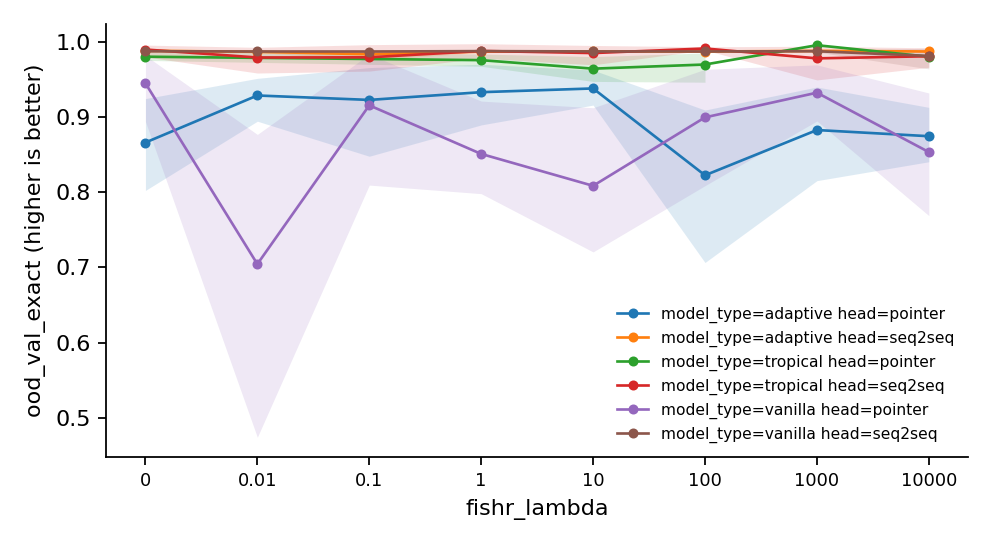
\includegraphics[width=\textwidth]{metric_ood_val_exact.png}
\caption{\texttt{ood\_val\_exact} against \texttt{fishr\_lambda}: the mean over seeds with a 95\% bootstrap CI, one line per combination of the other factors.}
\label{fig:ood_val_exact}
\end{figure}

{\small
\begin{longtable}{lllrlrrr}
\caption{\texttt{ood\_val\_exact} per cell: mean, 95\% bootstrap CI, SD, seeds, diverged runs.}\label{tab:summary-ood_val_exact}\\
\toprule
\texttt{model\_type} & \texttt{head} & \texttt{fishr\_lambda} & mean & 95\% CI & SD & $n$ & div.\\
\midrule
\endhead
adaptive & pointer & 0 & 0.8659 & [0.802, 0.924] & 0.0777 & 5 & 0\\
adaptive & pointer & 0.01 & 0.9285 & [0.894, 0.951] & 0.0383 & 5 & 0\\
adaptive & pointer & 0.1 & 0.9226 & [0.848, 0.966] & 0.0829 & 5 & 0\\
adaptive & pointer & 1 & 0.9329 & [0.889, 0.97] & 0.053 & 5 & 0\\
adaptive & pointer & 10 & 0.9378 & [0.916, 0.962] & 0.0291 & 5 & 0\\
adaptive & pointer & 100 & 0.8224 & [0.706, 0.909] & 0.137 & 5 & 0\\
adaptive & pointer & 1000 & 0.8825 & [0.815, 0.94] & 0.0808 & 5 & 0\\
adaptive & pointer & 1e+04 & 0.8743 & [0.84, 0.913] & 0.0478 & 5 & 0\\
adaptive & seq2seq & 0 & 0.988 & [0.986, 0.99] & 0.00281 & 5 & 0\\
adaptive & seq2seq & 0.01 & 0.9865 & [0.986, 0.987] & $9.54\times10^{-4}$ & 5 & 0\\
adaptive & seq2seq & 0.1 & 0.9833 & [0.976, 0.988] & 0.00841 & 5 & 0\\
adaptive & seq2seq & 1 & 0.9868 & [0.986, 0.988] & 0.00142 & 5 & 0\\
adaptive & seq2seq & 10 & 0.987 & [0.986, 0.988] & 0.00159 & 5 & 0\\
adaptive & seq2seq & 100 & 0.9869 & [0.986, 0.988] & 0.0016 & 5 & 0\\
adaptive & seq2seq & 1000 & 0.9877 & [0.986, 0.991] & 0.00304 & 5 & 0\\
adaptive & seq2seq & 1e+04 & 0.987 & [0.986, 0.988] & 0.00153 & 5 & 0\\
tropical & pointer & 0 & 0.98 & [0.975, 0.987] & 0.00669 & 4 & 0\\
tropical & pointer & 1 & 0.9755 & [0.967, 0.984] & 0.0115 & 2 & 0\\
tropical & pointer & 10 & 0.9641 & [0.947, 0.98] & 0.022 & 5 & 0\\
tropical & pointer & 100 & 0.9696 & [0.946, 0.985] & 0.0207 & 3 & 0\\
tropical & pointer & 1000 & 0.9953 & [--, --] & -- & 1 & 0\\
tropical & pointer & 1e+04 & 0.98 & [--, --] & -- & 1 & 0\\
tropical & seq2seq & 0 & 0.9896 & [0.98, 0.995] & 0.0108 & 5 & 0\\
tropical & seq2seq & 0.01 & 0.979 & [0.958, 0.992] & 0.0225 & 5 & 0\\
tropical & seq2seq & 0.1 & 0.9792 & [0.961, 0.996] & 0.0222 & 5 & 0\\
tropical & seq2seq & 1 & 0.9877 & [0.978, 0.997] & 0.0125 & 5 & 0\\
tropical & seq2seq & 10 & 0.9849 & [0.969, 0.995] & 0.018 & 5 & 0\\
tropical & seq2seq & 100 & 0.9909 & [0.989, 0.993] & 0.00281 & 5 & 0\\
tropical & seq2seq & 1000 & 0.9778 & [0.949, 0.994] & 0.032 & 5 & 0\\
tropical & seq2seq & 1e+04 & 0.9806 & [0.966, 0.992] & 0.0165 & 5 & 0\\
vanilla & pointer & 0 & 0.9447 & [0.894, 0.982] & 0.057 & 5 & 0\\
vanilla & pointer & 0.01 & 0.7043 & [0.474, 0.877] & 0.26 & 5 & 0\\
vanilla & pointer & 0.1 & 0.9154 & [0.809, 0.983] & 0.121 & 5 & 0\\
vanilla & pointer & 1 & 0.8508 & [0.798, 0.921] & 0.0796 & 5 & 0\\
vanilla & pointer & 10 & 0.8084 & [0.72, 0.912] & 0.124 & 5 & 0\\
vanilla & pointer & 100 & 0.8994 & [0.809, 0.963] & 0.104 & 5 & 0\\
vanilla & pointer & 1000 & 0.9322 & [0.895, 0.969] & 0.0494 & 5 & 0\\
vanilla & pointer & 1e+04 & 0.8532 & [0.769, 0.932] & 0.109 & 5 & 0\\
vanilla & seq2seq & 0 & 0.9873 & [0.986, 0.989] & 0.0018 & 5 & 0\\
vanilla & seq2seq & 0.01 & 0.987 & [0.986, 0.988] & 0.00153 & 5 & 0\\
vanilla & seq2seq & 0.1 & 0.9869 & [0.986, 0.988] & 0.00166 & 5 & 0\\
vanilla & seq2seq & 1 & 0.9874 & [0.986, 0.99] & 0.00248 & 5 & 0\\
vanilla & seq2seq & 10 & 0.987 & [0.986, 0.988] & 0.00162 & 5 & 0\\
vanilla & seq2seq & 100 & 0.987 & [0.986, 0.988] & 0.00153 & 5 & 0\\
vanilla & seq2seq & 1000 & 0.9873 & [0.986, 0.989] & 0.00166 & 5 & 0\\
vanilla & seq2seq & 1e+04 & 0.981 & [0.964, 0.991] & 0.0191 & 5 & 0\\
\bottomrule
\end{longtable}
}

{\small
\begin{longtable}{lllrrrl}
\caption{\texttt{ood\_val\_exact}: each level of \texttt{fishr\_lambda} against its control (0), within each combination of the other factors. parametric: Dunnett vs control.}\label{tab:control-ood_val_exact}\\
\toprule
\texttt{model\_type} & \texttt{head} & \texttt{fishr\_lambda} & difference & 95\% CI & $p$ & \\
\midrule
\endhead
adaptive & pointer & 0.01 & 0.06254 & [-0.0695, 0.195] & 0.6532 & \\
adaptive & pointer & 0.1 & 0.05664 & [-0.0754, 0.189] & 0.7395 & \\
adaptive & pointer & 1 & 0.06694 & [-0.0651, 0.199] & 0.5879 & \\
adaptive & pointer & 10 & 0.0719 & [-0.0602, 0.204] & 0.5158 & \\
adaptive & pointer & 100 & -0.04356 & [-0.176, 0.0885] & 0.8995 & \\
adaptive & pointer & 1000 & 0.0166 & [-0.115, 0.149] & 0.9995 & \\
adaptive & pointer & 1e+04 & 0.0084 & [-0.124, 0.14] & 1.0000 & \\
adaptive & seq2seq & 0.01 & -0.00146 & [-0.00758, 0.00466] & 0.9783 & \\
adaptive & seq2seq & 0.1 & -0.00468 & [-0.0108, 0.00144] & 0.1938 & \\
adaptive & seq2seq & 1 & -0.00112 & [-0.00724, 0.005] & 0.9951 & \\
adaptive & seq2seq & 10 & $-9.400\times10^{-4}$ & [-0.00706, 0.00518] & 0.9983 & \\
adaptive & seq2seq & 100 & -0.00104 & [-0.00716, 0.00508] & 0.9968 & \\
adaptive & seq2seq & 1000 & $-2.200\times10^{-4}$ & [-0.00634, 0.0059] & 1.0000 & \\
adaptive & seq2seq & 1e+04 & $-1.000\times10^{-3}$ & [-0.00712, 0.00512] & 0.9975 & \\
tropical & seq2seq & 0.01 & -0.0106 & [-0.0439, 0.0227] & 0.9133 & \\
tropical & seq2seq & 0.1 & -0.01036 & [-0.0436, 0.0229] & 0.9215 & \\
tropical & seq2seq & 1 & -0.00188 & [-0.0352, 0.0314] & 1.0000 & \\
tropical & seq2seq & 10 & -0.0047 & [-0.038, 0.0286] & 0.9990 & \\
tropical & seq2seq & 100 & 0.00138 & [-0.0319, 0.0347] & 1.0000 & \\
tropical & seq2seq & 1000 & -0.01174 & [-0.045, 0.0215] & 0.8683 & \\
tropical & seq2seq & 1e+04 & -0.00892 & [-0.0422, 0.0244] & 0.9608 & \\
vanilla & pointer & 0.01 & -0.2404 & [-0.465, -0.0158] & 0.0318 & *\\
vanilla & pointer & 0.1 & -0.02932 & [-0.254, 0.195] & 0.9994 & \\
vanilla & pointer & 1 & -0.09394 & [-0.319, 0.131] & 0.7592 & \\
vanilla & pointer & 10 & -0.1363 & [-0.361, 0.0883] & 0.4042 & \\
vanilla & pointer & 100 & -0.04534 & [-0.27, 0.179] & 0.9913 & \\
vanilla & pointer & 1000 & -0.01252 & [-0.237, 0.212] & 1.0000 & \\
vanilla & pointer & 1e+04 & -0.09146 & [-0.316, 0.133] & 0.7794 & \\
vanilla & seq2seq & 0.01 & $-3.600\times10^{-4}$ & [-0.0125, 0.0118] & 1.0000 & \\
vanilla & seq2seq & 0.1 & $-4.000\times10^{-4}$ & [-0.0125, 0.0117] & 1.0000 & \\
vanilla & seq2seq & 1 & $1.200\times10^{-4}$ & [-0.012, 0.0122] & 1.0000 & \\
vanilla & seq2seq & 10 & $-2.800\times10^{-4}$ & [-0.0124, 0.0118] & 1.0000 & \\
vanilla & seq2seq & 100 & $-3.600\times10^{-4}$ & [-0.0125, 0.0118] & 1.0000 & \\
vanilla & seq2seq & 1000 & 0 & [-0.0121, 0.0121] & 1.0000 & \\
vanilla & seq2seq & 1e+04 & -0.00628 & [-0.0184, 0.00584] & 0.5660 & \\
\bottomrule
\end{longtable}
}

{\small
\begin{longtable}{llrrrrr}
\caption{\texttt{ood\_val\_exact} against log10 \texttt{fishr\_lambda}: parametric: OLS slope t-test, seed-bootstrap CI, with the Jonckheere--Terpstra ordered-trend $\tau$ and $p$.}\label{tab:trend-ood_val_exact}\\
\toprule
\texttt{model\_type} & \texttt{head} & estimate & 95\% CI & $p$ & JT $\tau$ & JT $p$\\
\midrule
\endhead
adaptive & pointer & -0.01261 & [-0.019, -0.00626] & 0.0582 & -0.326 & 0.0124\\
adaptive & seq2seq & $3.707\times10^{-4}$ & [$5.71\times10^{-6}$, $8.78\times10^{-4}$] & 0.2198 & 0.0457 & 0.7387\\
tropical & pointer & 0.00405 & [$-1.80\times10^{-4}$, 0.0117] & 0.4300 & 0.154 & 0.6107\\
tropical & seq2seq & $1.979\times10^{-4}$ & [-0.00355, 0.00436] & 0.9026 & -0.0019 & 0.9952\\
vanilla & pointer & 0.0189 & [0.00502, 0.0328] & 0.1202 & 0.109 & 0.4333\\
vanilla & seq2seq & $-6.229\times10^{-4}$ & [-0.00233, $3.00\times10^{-4}$] & 0.3023 & 0.107 & 0.4105\\
\bottomrule
\end{longtable}
}

{\small
\begin{longtable}{lrrrl}
\caption{\texttt{ood\_val\_exact}: paired contrasts by seed, Holm-corrected across the cells. parametric: paired t-test by seed, Holm.}\label{tab:paired-ood_val_exact}\\
\toprule
contrast (within) & difference & 95\% CI & $p$ & \\
\midrule
\endhead
\stackcell{model\_type: tropical - vanilla\\\footnotesize head=pointer fishr\_lambda=0 } & 0.03252 & [-0.0818, 0.147] & 1.0000 & \\
\stackcell{model\_type: tropical - vanilla\\\footnotesize head=pointer fishr\_lambda=1 } & 0.1419 & [-0.115, 0.399] & 0.9027 & \\
\stackcell{model\_type: tropical - vanilla\\\footnotesize head=pointer fishr\_lambda=10 } & 0.1558 & [0.00905, 0.302] & 0.5048 & \\
\stackcell{model\_type: tropical - vanilla\\\footnotesize head=pointer fishr\_lambda=100 } & 0.1043 & [-0.166, 0.375] & 1.0000 & \\
\stackcell{model\_type: tropical - vanilla\\\footnotesize head=seq2seq fishr\_lambda=0 } & 0.00224 & [-0.0124, 0.0169] & 1.0000 & \\
\stackcell{model\_type: tropical - vanilla\\\footnotesize head=seq2seq fishr\_lambda=0.01 } & -0.008 & [-0.0375, 0.0215] & 1.0000 & \\
\stackcell{model\_type: tropical - vanilla\\\footnotesize head=seq2seq fishr\_lambda=0.1 } & -0.00772 & [-0.0369, 0.0214] & 1.0000 & \\
\stackcell{model\_type: tropical - vanilla\\\footnotesize head=seq2seq fishr\_lambda=1 } & $2.400\times10^{-4}$ & [-0.015, 0.0155] & 1.0000 & \\
\stackcell{model\_type: tropical - vanilla\\\footnotesize head=seq2seq fishr\_lambda=10 } & -0.00218 & [-0.0245, 0.0202] & 1.0000 & \\
\stackcell{model\_type: tropical - vanilla\\\footnotesize head=seq2seq fishr\_lambda=100 } & 0.00398 & [$-3.39\times10^{-4}$, 0.0083] & 0.6899 & \\
\stackcell{model\_type: tropical - vanilla\\\footnotesize head=seq2seq fishr\_lambda=1000 } & -0.0095 & [-0.049, 0.03] & 1.0000 & \\
\stackcell{model\_type: tropical - vanilla\\\footnotesize head=seq2seq fishr\_lambda=1e+04 } & $-4.000\times10^{-4}$ & [-0.0357, 0.0349] & 1.0000 & \\
\stackcell{model\_type: adaptive - vanilla\\\footnotesize head=pointer fishr\_lambda=0 } & -0.07878 & [-0.182, 0.0244] & 1.0000 & \\
\stackcell{model\_type: adaptive - vanilla\\\footnotesize head=pointer fishr\_lambda=0.01 } & 0.2242 & [-0.106, 0.555] & 1.0000 & \\
\stackcell{model\_type: adaptive - vanilla\\\footnotesize head=pointer fishr\_lambda=0.1 } & 0.00718 & [-0.209, 0.223] & 1.0000 & \\
\stackcell{model\_type: adaptive - vanilla\\\footnotesize head=pointer fishr\_lambda=1 } & 0.0821 & [-0.0755, 0.24] & 1.0000 & \\
\stackcell{model\_type: adaptive - vanilla\\\footnotesize head=pointer fishr\_lambda=10 } & 0.1295 & [-0.0368, 0.296] & 1.0000 & \\
\stackcell{model\_type: adaptive - vanilla\\\footnotesize head=pointer fishr\_lambda=100 } & -0.077 & [-0.149, -0.00476] & 0.6654 & \\
\stackcell{model\_type: adaptive - vanilla\\\footnotesize head=pointer fishr\_lambda=1000 } & -0.04966 & [-0.205, 0.106] & 1.0000 & \\
\stackcell{model\_type: adaptive - vanilla\\\footnotesize head=pointer fishr\_lambda=1e+04 } & 0.02108 & [-0.0973, 0.139] & 1.0000 & \\
\stackcell{model\_type: adaptive - vanilla\\\footnotesize head=seq2seq fishr\_lambda=0 } & $6.400\times10^{-4}$ & [-0.00121, 0.00249] & 1.0000 & \\
\stackcell{model\_type: adaptive - vanilla\\\footnotesize head=seq2seq fishr\_lambda=0.01 } & $-4.600\times10^{-4}$ & [-0.00175, $8.26\times10^{-4}$] & 1.0000 & \\
\stackcell{model\_type: adaptive - vanilla\\\footnotesize head=seq2seq fishr\_lambda=0.1 } & -0.00364 & [-0.0139, 0.00661] & 1.0000 & \\
\stackcell{model\_type: adaptive - vanilla\\\footnotesize head=seq2seq fishr\_lambda=1 } & $-6.000\times10^{-4}$ & [-0.00213, $9.33\times10^{-4}$] & 1.0000 & \\
\stackcell{model\_type: adaptive - vanilla\\\footnotesize head=seq2seq fishr\_lambda=10 } & $-2.000\times10^{-5}$ & [$-3.29\times10^{-4}$, $2.89\times10^{-4}$] & 1.0000 & \\
\stackcell{model\_type: adaptive - vanilla\\\footnotesize head=seq2seq fishr\_lambda=100 } & $-4.000\times10^{-5}$ & [$-1.51\times10^{-4}$, $7.11\times10^{-5}$] & 1.0000 & \\
\stackcell{model\_type: adaptive - vanilla\\\footnotesize head=seq2seq fishr\_lambda=1000 } & $4.200\times10^{-4}$ & [-0.00204, 0.00288] & 1.0000 & \\
\stackcell{model\_type: adaptive - vanilla\\\footnotesize head=seq2seq fishr\_lambda=1e+04 } & 0.00592 & [-0.0162, 0.0281] & 1.0000 & \\
\stackcell{head: pointer - seq2seq\\\footnotesize model\_type=adaptive fishr\_lambda=0 } & -0.122 & [-0.217, -0.0267] & 0.4026 & \\
\stackcell{head: pointer - seq2seq\\\footnotesize model\_type=adaptive fishr\_lambda=0.01 } & -0.05804 & [-0.106, -0.0104] & 0.4421 & \\
\stackcell{head: pointer - seq2seq\\\footnotesize model\_type=adaptive fishr\_lambda=0.1 } & -0.06072 & [-0.166, 0.0449] & 1.0000 & \\
\stackcell{head: pointer - seq2seq\\\footnotesize model\_type=adaptive fishr\_lambda=1 } & -0.05398 & [-0.119, 0.0107] & 0.7392 & \\
\stackcell{head: pointer - seq2seq\\\footnotesize model\_type=adaptive fishr\_lambda=10 } & -0.0492 & [-0.0844, -0.014] & 0.3396 & \\
\stackcell{head: pointer - seq2seq\\\footnotesize model\_type=adaptive fishr\_lambda=100 } & -0.1646 & [-0.337, 0.0075] & 0.6800 & \\
\stackcell{head: pointer - seq2seq\\\footnotesize model\_type=adaptive fishr\_lambda=1000 } & -0.1052 & [-0.204, -0.00656] & 0.5811 & \\
\stackcell{head: pointer - seq2seq\\\footnotesize model\_type=adaptive fishr\_lambda=1e+04 } & -0.1126 & [-0.17, -0.0549] & 0.1124 & \\
\stackcell{head: pointer - seq2seq\\\footnotesize model\_type=tropical fishr\_lambda=0 } & -0.008375 & [-0.0256, 0.00885] & 1.0000 & \\
\stackcell{head: pointer - seq2seq\\\footnotesize model\_type=tropical fishr\_lambda=1 } & 0.0011 & [-0.0739, 0.0761] & 1.0000 & \\
\stackcell{head: pointer - seq2seq\\\footnotesize model\_type=tropical fishr\_lambda=10 } & -0.02074 & [-0.0655, 0.0241] & 1.0000 & \\
\stackcell{head: pointer - seq2seq\\\footnotesize model\_type=tropical fishr\_lambda=100 } & -0.02267 & [-0.0754, 0.03] & 1.0000 & \\
\stackcell{head: pointer - seq2seq\\\footnotesize model\_type=vanilla fishr\_lambda=0 } & -0.04262 & [-0.113, 0.0283] & 1.0000 & \\
\stackcell{head: pointer - seq2seq\\\footnotesize model\_type=vanilla fishr\_lambda=0.01 } & -0.2827 & [-0.604, 0.0386] & 0.7392 & \\
\stackcell{head: pointer - seq2seq\\\footnotesize model\_type=vanilla fishr\_lambda=0.1 } & -0.07154 & [-0.223, 0.0796] & 1.0000 & \\
\stackcell{head: pointer - seq2seq\\\footnotesize model\_type=vanilla fishr\_lambda=1 } & -0.1367 & [-0.238, -0.0353] & 0.3611 & \\
\stackcell{head: pointer - seq2seq\\\footnotesize model\_type=vanilla fishr\_lambda=10 } & -0.1787 & [-0.332, -0.0255] & 0.4755 & \\
\stackcell{head: pointer - seq2seq\\\footnotesize model\_type=vanilla fishr\_lambda=100 } & -0.0876 & [-0.218, 0.0433] & 1.0000 & \\
\stackcell{head: pointer - seq2seq\\\footnotesize model\_type=vanilla fishr\_lambda=1000 } & -0.05514 & [-0.117, 0.00625] & 0.7392 & \\
\stackcell{head: pointer - seq2seq\\\footnotesize model\_type=vanilla fishr\_lambda=1e+04 } & -0.1278 & [-0.251, -0.0049] & 0.5811 & \\
\bottomrule
\end{longtable}
}

\subsection{\texttt{ood\_noise\_f1}}
\begin{figure}[tbp]
\centering
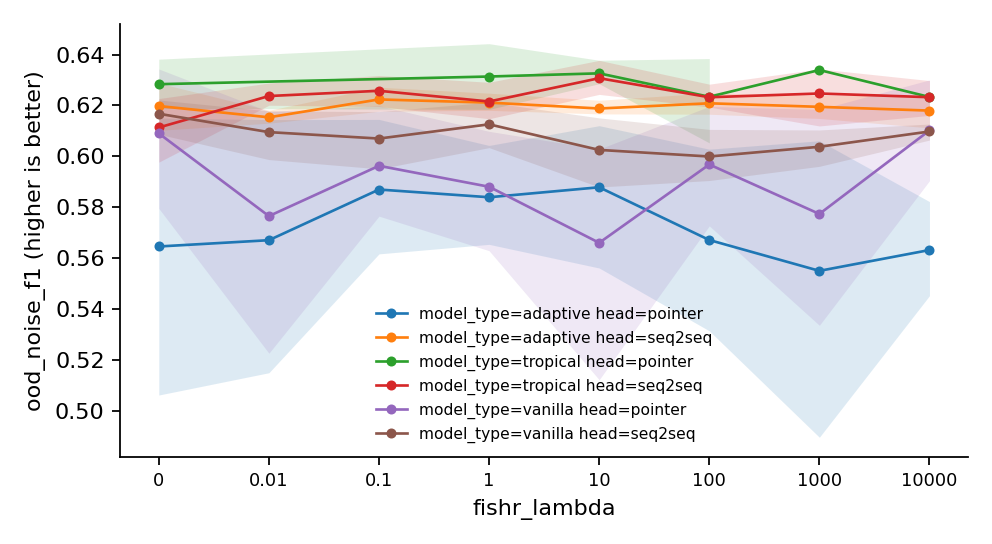
\includegraphics[width=\textwidth]{metric_ood_noise_f1.png}
\caption{\texttt{ood\_noise\_f1} against \texttt{fishr\_lambda}: the mean over seeds with a 95\% bootstrap CI, one line per combination of the other factors.}
\label{fig:ood_noise_f1}
\end{figure}

{\small
\begin{longtable}{lllrlrrr}
\caption{\texttt{ood\_noise\_f1} per cell: mean, 95\% bootstrap CI, SD, seeds, diverged runs.}\label{tab:summary-ood_noise_f1}\\
\toprule
\texttt{model\_type} & \texttt{head} & \texttt{fishr\_lambda} & mean & 95\% CI & SD & $n$ & div.\\
\midrule
\endhead
adaptive & pointer & 0 & 0.5646 & [0.506, 0.615] & 0.0692 & 5 & 0\\
adaptive & pointer & 0.01 & 0.5671 & [0.515, 0.614] & 0.0644 & 5 & 0\\
adaptive & pointer & 0.1 & 0.587 & [0.562, 0.615] & 0.0344 & 5 & 0\\
adaptive & pointer & 1 & 0.5839 & [0.565, 0.604] & 0.0265 & 5 & 0\\
adaptive & pointer & 10 & 0.5879 & [0.556, 0.612] & 0.037 & 5 & 0\\
adaptive & pointer & 100 & 0.5671 & [0.531, 0.603] & 0.0487 & 5 & 0\\
adaptive & pointer & 1000 & 0.555 & [0.49, 0.606] & 0.0787 & 5 & 0\\
adaptive & pointer & 1e+04 & 0.5632 & [0.545, 0.582] & 0.024 & 5 & 0\\
adaptive & seq2seq & 0 & 0.6198 & [0.61, 0.629] & 0.012 & 5 & 0\\
adaptive & seq2seq & 0.01 & 0.6154 & [0.613, 0.618] & 0.00321 & 5 & 0\\
adaptive & seq2seq & 0.1 & 0.6224 & [0.618, 0.627] & 0.00565 & 5 & 0\\
adaptive & seq2seq & 1 & 0.6211 & [0.618, 0.625] & 0.00434 & 5 & 0\\
adaptive & seq2seq & 10 & 0.6188 & [0.617, 0.622] & 0.0037 & 5 & 0\\
adaptive & seq2seq & 100 & 0.6209 & [0.617, 0.625] & 0.00555 & 5 & 0\\
adaptive & seq2seq & 1000 & 0.6195 & [0.615, 0.624] & 0.0061 & 5 & 0\\
adaptive & seq2seq & 1e+04 & 0.618 & [0.611, 0.624] & 0.00803 & 5 & 0\\
tropical & pointer & 0 & 0.6284 & [0.619, 0.638] & 0.0106 & 4 & 0\\
tropical & pointer & 1 & 0.6314 & [0.618, 0.644] & 0.0183 & 2 & 0\\
tropical & pointer & 10 & 0.6326 & [0.629, 0.638] & 0.00621 & 5 & 0\\
tropical & pointer & 100 & 0.6234 & [0.605, 0.638] & 0.0168 & 3 & 0\\
tropical & pointer & 1000 & 0.6339 & [--, --] & -- & 1 & 0\\
tropical & pointer & 1e+04 & 0.6233 & [--, --] & -- & 1 & 0\\
tropical & seq2seq & 0 & 0.6114 & [0.598, 0.623] & 0.0157 & 5 & 0\\
tropical & seq2seq & 0.01 & 0.6237 & [0.62, 0.629] & 0.00557 & 5 & 0\\
tropical & seq2seq & 0.1 & 0.6258 & [0.62, 0.632] & 0.00805 & 5 & 0\\
tropical & seq2seq & 1 & 0.6216 & [0.615, 0.629] & 0.00946 & 5 & 0\\
tropical & seq2seq & 10 & 0.6307 & [0.624, 0.638] & 0.00872 & 5 & 0\\
tropical & seq2seq & 100 & 0.6232 & [0.619, 0.628] & 0.00602 & 5 & 0\\
tropical & seq2seq & 1000 & 0.6247 & [0.612, 0.634] & 0.0141 & 5 & 0\\
tropical & seq2seq & 1e+04 & 0.6233 & [0.616, 0.63] & 0.00926 & 5 & 0\\
vanilla & pointer & 0 & 0.609 & [0.58, 0.634] & 0.0357 & 5 & 0\\
vanilla & pointer & 0.01 & 0.5765 & [0.523, 0.618] & 0.0612 & 5 & 0\\
vanilla & pointer & 0.1 & 0.5963 & [0.577, 0.62] & 0.0273 & 5 & 0\\
vanilla & pointer & 1 & 0.5881 & [0.563, 0.61] & 0.0295 & 5 & 0\\
vanilla & pointer & 10 & 0.566 & [0.512, 0.603] & 0.0621 & 5 & 0\\
vanilla & pointer & 100 & 0.5968 & [0.573, 0.62] & 0.0321 & 5 & 0\\
vanilla & pointer & 1000 & 0.5774 & [0.534, 0.618] & 0.0524 & 5 & 0\\
vanilla & pointer & 1e+04 & 0.6102 & [0.59, 0.63] & 0.0262 & 5 & 0\\
vanilla & seq2seq & 0 & 0.6168 & [0.609, 0.622] & 0.00918 & 5 & 0\\
vanilla & seq2seq & 0.01 & 0.6095 & [0.599, 0.618] & 0.0123 & 5 & 0\\
vanilla & seq2seq & 0.1 & 0.607 & [0.595, 0.618] & 0.0145 & 5 & 0\\
vanilla & seq2seq & 1 & 0.6126 & [0.603, 0.621] & 0.0115 & 5 & 0\\
vanilla & seq2seq & 10 & 0.6025 & [0.588, 0.615] & 0.0175 & 5 & 0\\
vanilla & seq2seq & 100 & 0.6 & [0.591, 0.611] & 0.0132 & 5 & 0\\
vanilla & seq2seq & 1000 & 0.6038 & [0.596, 0.61] & 0.00953 & 5 & 0\\
vanilla & seq2seq & 1e+04 & 0.6098 & [0.606, 0.613] & 0.00396 & 5 & 0\\
\bottomrule
\end{longtable}
}

{\small
\begin{longtable}{lllrrrl}
\caption{\texttt{ood\_noise\_f1}: each level of \texttt{fishr\_lambda} against its control (0), within each combination of the other factors. parametric: Dunnett vs control.}\label{tab:control-ood_noise_f1}\\
\toprule
\texttt{model\_type} & \texttt{head} & \texttt{fishr\_lambda} & difference & 95\% CI & $p$ & \\
\midrule
\endhead
adaptive & pointer & 0.01 & 0.002471 & [-0.0877, 0.0927] & 1.0000 & \\
adaptive & pointer & 0.1 & 0.02239 & [-0.0678, 0.113] & 0.9734 & \\
adaptive & pointer & 1 & 0.01935 & [-0.0709, 0.11] & 0.9877 & \\
adaptive & pointer & 10 & 0.02327 & [-0.0669, 0.113] & 0.9676 & \\
adaptive & pointer & 100 & 0.002544 & [-0.0877, 0.0928] & 1.0000 & \\
adaptive & pointer & 1000 & -0.00958 & [-0.0998, 0.0806] & 0.9998 & \\
adaptive & pointer & 1e+04 & -0.001395 & [-0.0916, 0.0888] & 1.0000 & \\
adaptive & seq2seq & 0.01 & -0.004424 & [-0.016, 0.00715] & 0.8224 & \\
adaptive & seq2seq & 0.1 & 0.002599 & [-0.00898, 0.0142] & 0.9843 & \\
adaptive & seq2seq & 1 & 0.001348 & [-0.0102, 0.0129] & 0.9997 & \\
adaptive & seq2seq & 10 & $-9.646\times10^{-4}$ & [-0.0125, 0.0106] & 1.0000 & \\
adaptive & seq2seq & 100 & 0.001082 & [-0.0105, 0.0127] & 0.9999 & \\
adaptive & seq2seq & 1000 & $-3.135\times10^{-4}$ & [-0.0119, 0.0113] & 1.0000 & \\
adaptive & seq2seq & 1e+04 & -0.00179 & [-0.0134, 0.00979] & 0.9982 & \\
tropical & seq2seq & 0.01 & 0.01236 & [-0.00543, 0.0302] & 0.2735 & \\
tropical & seq2seq & 0.1 & 0.01442 & [-0.00337, 0.0322] & 0.1518 & \\
tropical & seq2seq & 1 & 0.01021 & [-0.00758, 0.028] & 0.4612 & \\
tropical & seq2seq & 10 & 0.01938 & [0.00159, 0.0372] & 0.0281 & *\\
tropical & seq2seq & 100 & 0.01188 & [-0.00591, 0.0297] & 0.3100 & \\
tropical & seq2seq & 1000 & 0.01336 & [-0.00443, 0.0312] & 0.2075 & \\
tropical & seq2seq & 1e+04 & 0.01191 & [-0.00588, 0.0297] & 0.3079 & \\
vanilla & pointer & 0.01 & -0.03251 & [-0.108, 0.043] & 0.7367 & \\
vanilla & pointer & 0.1 & -0.01274 & [-0.0883, 0.0628] & 0.9970 & \\
vanilla & pointer & 1 & -0.02097 & [-0.0965, 0.0546] & 0.9536 & \\
vanilla & pointer & 10 & -0.04301 & [-0.119, 0.0325] & 0.4698 & \\
vanilla & pointer & 100 & -0.01222 & [-0.0878, 0.0633] & 0.9976 & \\
vanilla & pointer & 1000 & -0.03166 & [-0.107, 0.0439] & 0.7576 & \\
vanilla & pointer & 1e+04 & 0.001165 & [-0.0744, 0.0767] & 1.0000 & \\
vanilla & seq2seq & 0.01 & -0.007223 & [-0.0283, 0.0138] & 0.8823 & \\
vanilla & seq2seq & 0.1 & -0.009749 & [-0.0308, 0.0113] & 0.6743 & \\
vanilla & seq2seq & 1 & -0.004158 & [-0.0252, 0.0169] & 0.9923 & \\
vanilla & seq2seq & 10 & -0.01421 & [-0.0353, 0.00685] & 0.3005 & \\
vanilla & seq2seq & 100 & -0.0168 & [-0.0379, 0.00427] & 0.1631 & \\
vanilla & seq2seq & 1000 & -0.01298 & [-0.034, 0.00809] & 0.3888 & \\
vanilla & seq2seq & 1e+04 & -0.006973 & [-0.028, 0.0141] & 0.8981 & \\
\bottomrule
\end{longtable}
}

{\small
\begin{longtable}{llrrrrr}
\caption{\texttt{ood\_noise\_f1} against log10 \texttt{fishr\_lambda}: parametric: OLS slope t-test, seed-bootstrap CI, with the Jonckheere--Terpstra ordered-trend $\tau$ and $p$.}\label{tab:trend-ood_noise_f1}\\
\toprule
\texttt{model\_type} & \texttt{head} & estimate & 95\% CI & $p$ & JT $\tau$ & JT $p$\\
\midrule
\endhead
adaptive & pointer & -0.003298 & [-0.00764, 0.00113] & 0.4023 & -0.173 & 0.1958\\
adaptive & seq2seq & $6.475\times10^{-5}$ & [$-6.35\times10^{-4}$, $7.42\times10^{-4}$] & 0.8897 & 0.0743 & 0.5867\\
tropical & pointer & -0.002089 & [-0.0128, 0.00124] & 0.4790 & -0.231 & 0.4419\\
tropical & seq2seq & $-6.474\times10^{-5}$ & [$-3.53\times10^{-4}$, $2.47\times10^{-4}$] & 0.9317 & 0.0324 & 0.8212\\
vanilla & pointer & 0.002569 & [-0.00149, 0.00619] & 0.4834 & 0.0552 & 0.6937\\
vanilla & seq2seq & $-6.557\times10^{-4}$ & [-0.00182, $6.71\times10^{-4}$] & 0.5276 & -0.101 & 0.4469\\
\bottomrule
\end{longtable}
}

{\small
\begin{longtable}{lrrrl}
\caption{\texttt{ood\_noise\_f1}: paired contrasts by seed, Holm-corrected across the cells. parametric: paired t-test by seed, Holm.}\label{tab:paired-ood_noise_f1}\\
\toprule
contrast (within) & difference & 95\% CI & $p$ & \\
\midrule
\endhead
\stackcell{model\_type: tropical - vanilla\\\footnotesize head=pointer fishr\_lambda=0 } & 0.01566 & [-0.0382, 0.0695] & 1.0000 & \\
\stackcell{model\_type: tropical - vanilla\\\footnotesize head=pointer fishr\_lambda=1 } & 0.04924 & [-0.566, 0.665] & 1.0000 & \\
\stackcell{model\_type: tropical - vanilla\\\footnotesize head=pointer fishr\_lambda=10 } & 0.06661 & [-0.0108, 0.144] & 0.5689 & \\
\stackcell{model\_type: tropical - vanilla\\\footnotesize head=pointer fishr\_lambda=100 } & 0.02913 & [-0.0672, 0.125] & 1.0000 & \\
\stackcell{model\_type: tropical - vanilla\\\footnotesize head=seq2seq fishr\_lambda=0 } & -0.005399 & [-0.0188, 0.00801] & 1.0000 & \\
\stackcell{model\_type: tropical - vanilla\\\footnotesize head=seq2seq fishr\_lambda=0.01 } & 0.01419 & [-0.00195, 0.0303] & 0.5689 & \\
\stackcell{model\_type: tropical - vanilla\\\footnotesize head=seq2seq fishr\_lambda=0.1 } & 0.01877 & [-0.0077, 0.0452] & 0.7221 & \\
\stackcell{model\_type: tropical - vanilla\\\footnotesize head=seq2seq fishr\_lambda=1 } & 0.008972 & [-0.0057, 0.0236] & 0.8238 & \\
\stackcell{model\_type: tropical - vanilla\\\footnotesize head=seq2seq fishr\_lambda=10 } & 0.02819 & [0.0083, 0.0481] & 0.1704 & \\
\stackcell{model\_type: tropical - vanilla\\\footnotesize head=seq2seq fishr\_lambda=100 } & 0.02328 & [0.00842, 0.0381] & 0.1338 & \\
\stackcell{model\_type: tropical - vanilla\\\footnotesize head=seq2seq fishr\_lambda=1000 } & 0.02094 & [-0.00129, 0.0432] & 0.5316 & \\
\stackcell{model\_type: tropical - vanilla\\\footnotesize head=seq2seq fishr\_lambda=1e+04 } & 0.01348 & [0.00657, 0.0204] & 0.0677 & \\
\stackcell{model\_type: adaptive - vanilla\\\footnotesize head=pointer fishr\_lambda=0 } & -0.04445 & [-0.126, 0.0372] & 1.0000 & \\
\stackcell{model\_type: adaptive - vanilla\\\footnotesize head=pointer fishr\_lambda=0.01 } & -0.009471 & [-0.146, 0.127] & 1.0000 & \\
\stackcell{model\_type: adaptive - vanilla\\\footnotesize head=pointer fishr\_lambda=0.1 } & -0.009324 & [-0.0684, 0.0498] & 1.0000 & \\
\stackcell{model\_type: adaptive - vanilla\\\footnotesize head=pointer fishr\_lambda=1 } & -0.004125 & [-0.0532, 0.0449] & 1.0000 & \\
\stackcell{model\_type: adaptive - vanilla\\\footnotesize head=pointer fishr\_lambda=10 } & 0.02183 & [-0.0728, 0.116] & 1.0000 & \\
\stackcell{model\_type: adaptive - vanilla\\\footnotesize head=pointer fishr\_lambda=100 } & -0.02969 & [-0.079, 0.0196] & 1.0000 & \\
\stackcell{model\_type: adaptive - vanilla\\\footnotesize head=pointer fishr\_lambda=1000 } & -0.02237 & [-0.179, 0.135] & 1.0000 & \\
\stackcell{model\_type: adaptive - vanilla\\\footnotesize head=pointer fishr\_lambda=1e+04 } & -0.04701 & [-0.0949, $8.93\times10^{-4}$] & 0.7382 & \\
\stackcell{model\_type: adaptive - vanilla\\\footnotesize head=seq2seq fishr\_lambda=0 } & 0.003029 & [-0.018, 0.0241] & 1.0000 & \\
\stackcell{model\_type: adaptive - vanilla\\\footnotesize head=seq2seq fishr\_lambda=0.01 } & 0.005828 & [-0.00704, 0.0187] & 1.0000 & \\
\stackcell{model\_type: adaptive - vanilla\\\footnotesize head=seq2seq fishr\_lambda=0.1 } & 0.01538 & [-0.00642, 0.0372] & 1.0000 & \\
\stackcell{model\_type: adaptive - vanilla\\\footnotesize head=seq2seq fishr\_lambda=1 } & 0.008535 & [-0.00558, 0.0226] & 1.0000 & \\
\stackcell{model\_type: adaptive - vanilla\\\footnotesize head=seq2seq fishr\_lambda=10 } & 0.01628 & [-0.00945, 0.042] & 1.0000 & \\
\stackcell{model\_type: adaptive - vanilla\\\footnotesize head=seq2seq fishr\_lambda=100 } & 0.02091 & [0.00318, 0.0386] & 0.4909 & \\
\stackcell{model\_type: adaptive - vanilla\\\footnotesize head=seq2seq fishr\_lambda=1000 } & 0.0157 & [0.00221, 0.0292] & 0.4909 & \\
\stackcell{model\_type: adaptive - vanilla\\\footnotesize head=seq2seq fishr\_lambda=1e+04 } & 0.008213 & [$-2.50\times10^{-4}$, 0.0167] & 0.7382 & \\
\stackcell{head: pointer - seq2seq\\\footnotesize model\_type=adaptive fishr\_lambda=0 } & -0.0552 & [-0.138, 0.0279] & 1.0000 & \\
\stackcell{head: pointer - seq2seq\\\footnotesize model\_type=adaptive fishr\_lambda=0.01 } & -0.04831 & [-0.129, 0.0323] & 1.0000 & \\
\stackcell{head: pointer - seq2seq\\\footnotesize model\_type=adaptive fishr\_lambda=0.1 } & -0.03541 & [-0.079, 0.00815] & 1.0000 & \\
\stackcell{head: pointer - seq2seq\\\footnotesize model\_type=adaptive fishr\_lambda=1 } & -0.0372 & [-0.0724, -0.00194] & 0.8139 & \\
\stackcell{head: pointer - seq2seq\\\footnotesize model\_type=adaptive fishr\_lambda=10 } & -0.03096 & [-0.0775, 0.0156] & 1.0000 & \\
\stackcell{head: pointer - seq2seq\\\footnotesize model\_type=adaptive fishr\_lambda=100 } & -0.05374 & [-0.11, 0.00302] & 1.0000 & \\
\stackcell{head: pointer - seq2seq\\\footnotesize model\_type=adaptive fishr\_lambda=1000 } & -0.06447 & [-0.16, 0.0309] & 1.0000 & \\
\stackcell{head: pointer - seq2seq\\\footnotesize model\_type=adaptive fishr\_lambda=1e+04 } & -0.05481 & [-0.0831, -0.0265] & 0.1154 & \\
\stackcell{head: pointer - seq2seq\\\footnotesize model\_type=tropical fishr\_lambda=0 } & 0.01506 & [-0.0143, 0.0444] & 1.0000 & \\
\stackcell{head: pointer - seq2seq\\\footnotesize model\_type=tropical fishr\_lambda=1 } & 0.01771 & [-0.113, 0.148] & 1.0000 & \\
\stackcell{head: pointer - seq2seq\\\footnotesize model\_type=tropical fishr\_lambda=10 } & 0.001906 & [-0.00531, 0.00912] & 1.0000 & \\
\stackcell{head: pointer - seq2seq\\\footnotesize model\_type=tropical fishr\_lambda=100 } & 0.003322 & [-0.0459, 0.0526] & 1.0000 & \\
\stackcell{head: pointer - seq2seq\\\footnotesize model\_type=vanilla fishr\_lambda=0 } & -0.007723 & [-0.0595, 0.0441] & 1.0000 & \\
\stackcell{head: pointer - seq2seq\\\footnotesize model\_type=vanilla fishr\_lambda=0.01 } & -0.03301 & [-0.109, 0.0435] & 1.0000 & \\
\stackcell{head: pointer - seq2seq\\\footnotesize model\_type=vanilla fishr\_lambda=0.1 } & -0.01071 & [-0.0565, 0.0351] & 1.0000 & \\
\stackcell{head: pointer - seq2seq\\\footnotesize model\_type=vanilla fishr\_lambda=1 } & -0.02454 & [-0.0633, 0.0142] & 1.0000 & \\
\stackcell{head: pointer - seq2seq\\\footnotesize model\_type=vanilla fishr\_lambda=10 } & -0.03652 & [-0.0964, 0.0234] & 1.0000 & \\
\stackcell{head: pointer - seq2seq\\\footnotesize model\_type=vanilla fishr\_lambda=100 } & -0.003142 & [-0.0459, 0.0396] & 1.0000 & \\
\stackcell{head: pointer - seq2seq\\\footnotesize model\_type=vanilla fishr\_lambda=1000 } & -0.0264 & [-0.0807, 0.0279] & 1.0000 & \\
\stackcell{head: pointer - seq2seq\\\footnotesize model\_type=vanilla fishr\_lambda=1e+04 } & $4.157\times10^{-4}$ & [-0.0298, 0.0307] & 1.0000 & \\
\bottomrule
\end{longtable}
}

\subsection{\texttt{ood\_noise\_exact}}
\begin{figure}[tbp]
\centering
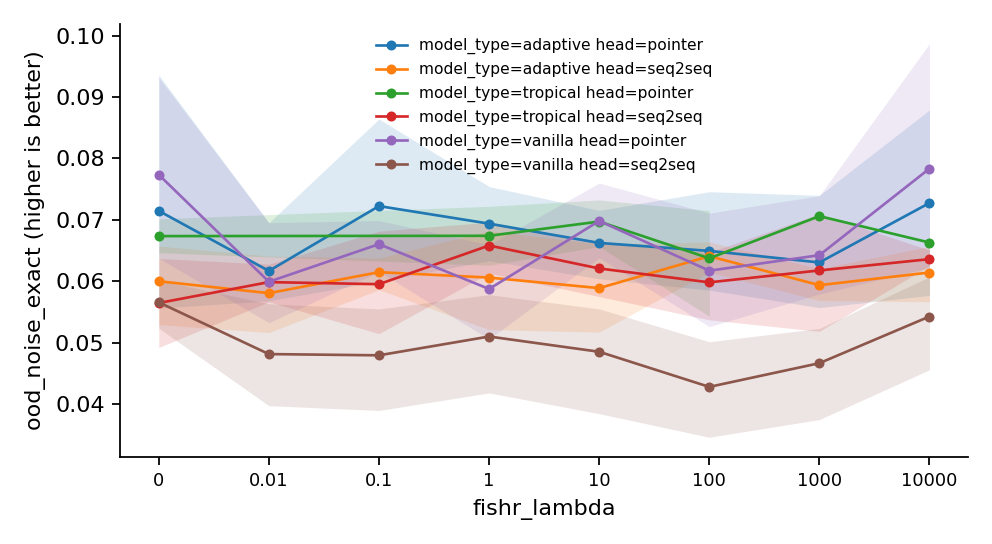
\includegraphics[width=\textwidth]{metric_ood_noise_exact.png}
\caption{\texttt{ood\_noise\_exact} against \texttt{fishr\_lambda}: the mean over seeds with a 95\% bootstrap CI, one line per combination of the other factors.}
\label{fig:ood_noise_exact}
\end{figure}

{\small
\begin{longtable}{lllrlrrr}
\caption{\texttt{ood\_noise\_exact} per cell: mean, 95\% bootstrap CI, SD, seeds, diverged runs.}\label{tab:summary-ood_noise_exact}\\
\toprule
\texttt{model\_type} & \texttt{head} & \texttt{fishr\_lambda} & mean & 95\% CI & SD & $n$ & div.\\
\midrule
\endhead
adaptive & pointer & 0 & 0.07146 & [0.0556, 0.0936] & 0.0246 & 5 & 0\\
adaptive & pointer & 0.01 & 0.06168 & [0.0568, 0.0695] & 0.00866 & 5 & 0\\
adaptive & pointer & 0.1 & 0.07224 & [0.06, 0.0864] & 0.0166 & 5 & 0\\
adaptive & pointer & 1 & 0.06938 & [0.0633, 0.0754] & 0.00768 & 5 & 0\\
adaptive & pointer & 10 & 0.06624 & [0.0604, 0.0715] & 0.00722 & 5 & 0\\
adaptive & pointer & 100 & 0.06494 & [0.0586, 0.0746] & 0.0108 & 5 & 0\\
adaptive & pointer & 1000 & 0.06306 & [0.0557, 0.074] & 0.0123 & 5 & 0\\
adaptive & pointer & 1e+04 & 0.07274 & [0.0577, 0.0879] & 0.0203 & 5 & 0\\
adaptive & seq2seq & 0 & 0.06 & [0.0529, 0.0657] & 0.00841 & 5 & 0\\
adaptive & seq2seq & 0.01 & 0.05806 & [0.0516, 0.0641] & 0.00811 & 5 & 0\\
adaptive & seq2seq & 0.1 & 0.06148 & [0.0586, 0.0638] & 0.00333 & 5 & 0\\
adaptive & seq2seq & 1 & 0.0606 & [0.0521, 0.0682] & 0.0103 & 5 & 0\\
adaptive & seq2seq & 10 & 0.05888 & [0.0517, 0.0661] & 0.00921 & 5 & 0\\
adaptive & seq2seq & 100 & 0.06408 & [0.0615, 0.0664] & 0.00337 & 5 & 0\\
adaptive & seq2seq & 1000 & 0.05936 & [0.0569, 0.0621] & 0.00337 & 5 & 0\\
adaptive & seq2seq & 1e+04 & 0.06142 & [0.0567, 0.0657] & 0.0058 & 5 & 0\\
tropical & pointer & 0 & 0.06735 & [0.0646, 0.0702] & 0.00352 & 4 & 0\\
tropical & pointer & 1 & 0.0674 & [0.0626, 0.0722] & 0.00679 & 2 & 0\\
tropical & pointer & 10 & 0.06972 & [0.0657, 0.0732] & 0.00485 & 5 & 0\\
tropical & pointer & 100 & 0.06373 & [0.0543, 0.0715] & 0.00872 & 3 & 0\\
tropical & pointer & 1000 & 0.0706 & [--, --] & -- & 1 & 0\\
tropical & pointer & 1e+04 & 0.0663 & [--, --] & -- & 1 & 0\\
tropical & seq2seq & 0 & 0.05646 & [0.0492, 0.0637] & 0.00972 & 5 & 0\\
tropical & seq2seq & 0.01 & 0.05986 & [0.0567, 0.0628] & 0.00403 & 5 & 0\\
tropical & seq2seq & 0.1 & 0.05952 & [0.0515, 0.0682] & 0.0109 & 5 & 0\\
tropical & seq2seq & 1 & 0.06582 & [0.0613, 0.0696] & 0.00542 & 5 & 0\\
tropical & seq2seq & 10 & 0.06208 & [0.0575, 0.0663] & 0.00563 & 5 & 0\\
tropical & seq2seq & 100 & 0.05982 & [0.0537, 0.0647] & 0.00691 & 5 & 0\\
tropical & seq2seq & 1000 & 0.06176 & [0.0518, 0.071] & 0.0127 & 5 & 0\\
tropical & seq2seq & 1e+04 & 0.0636 & [0.0625, 0.0651] & 0.00162 & 5 & 0\\
vanilla & pointer & 0 & 0.07734 & [0.0637, 0.0932] & 0.0191 & 5 & 0\\
vanilla & pointer & 0.01 & 0.05992 & [0.0533, 0.0695] & 0.0107 & 5 & 0\\
vanilla & pointer & 0.1 & 0.06604 & [0.0616, 0.0699] & 0.00561 & 5 & 0\\
vanilla & pointer & 1 & 0.05874 & [0.0506, 0.0659] & 0.00999 & 5 & 0\\
vanilla & pointer & 10 & 0.06982 & [0.0638, 0.076] & 0.00791 & 5 & 0\\
vanilla & pointer & 100 & 0.06172 & [0.0526, 0.0711] & 0.0121 & 5 & 0\\
vanilla & pointer & 1000 & 0.06424 & [0.0579, 0.0739] & 0.011 & 5 & 0\\
vanilla & pointer & 1e+04 & 0.07834 & [0.0622, 0.0987] & 0.0247 & 5 & 0\\
vanilla & seq2seq & 0 & 0.05656 & [0.0523, 0.0602] & 0.00506 & 5 & 0\\
vanilla & seq2seq & 0.01 & 0.04814 & [0.0397, 0.0563] & 0.0108 & 5 & 0\\
vanilla & seq2seq & 0.1 & 0.04794 & [0.039, 0.0555] & 0.0106 & 5 & 0\\
vanilla & seq2seq & 1 & 0.051 & [0.0418, 0.0578] & 0.0108 & 5 & 0\\
vanilla & seq2seq & 10 & 0.04852 & [0.0384, 0.0555] & 0.0114 & 5 & 0\\
vanilla & seq2seq & 100 & 0.0428 & [0.0346, 0.0502] & 0.0101 & 5 & 0\\
vanilla & seq2seq & 1000 & 0.04666 & [0.0375, 0.0523] & 0.00992 & 5 & 0\\
vanilla & seq2seq & 1e+04 & 0.05426 & [0.0456, 0.0607] & 0.00957 & 5 & 0\\
\bottomrule
\end{longtable}
}

{\small
\begin{longtable}{lllrrrl}
\caption{\texttt{ood\_noise\_exact}: each level of \texttt{fishr\_lambda} against its control (0), within each combination of the other factors. parametric: Dunnett vs control.}\label{tab:control-ood_noise_exact}\\
\toprule
\texttt{model\_type} & \texttt{head} & \texttt{fishr\_lambda} & difference & 95\% CI & $p$ & \\
\midrule
\endhead
adaptive & pointer & 0.01 & -0.00978 & [-0.0356, 0.016] & 0.8280 & \\
adaptive & pointer & 0.1 & $7.800\times10^{-4}$ & [-0.025, 0.0266] & 1.0000 & \\
adaptive & pointer & 1 & -0.00208 & [-0.0279, 0.0237] & 1.0000 & \\
adaptive & pointer & 10 & -0.00522 & [-0.031, 0.0206] & 0.9912 & \\
adaptive & pointer & 100 & -0.00652 & [-0.0323, 0.0193] & 0.9709 & \\
adaptive & pointer & 1000 & -0.0084 & [-0.0342, 0.0174] & 0.9051 & \\
adaptive & pointer & 1e+04 & 0.00128 & [-0.0245, 0.0271] & 1.0000 & \\
adaptive & seq2seq & 0.01 & -0.00194 & [-0.0142, 0.0103] & 0.9980 & \\
adaptive & seq2seq & 0.1 & 0.00148 & [-0.0108, 0.0138] & 0.9996 & \\
adaptive & seq2seq & 1 & $6.000\times10^{-4}$ & [-0.0117, 0.0129] & 1.0000 & \\
adaptive & seq2seq & 10 & -0.00112 & [-0.0134, 0.0112] & 0.9999 & \\
adaptive & seq2seq & 100 & 0.00408 & [-0.0082, 0.0164] & 0.8964 & \\
adaptive & seq2seq & 1000 & $-6.400\times10^{-4}$ & [-0.0129, 0.0116] & 1.0000 & \\
adaptive & seq2seq & 1e+04 & 0.00142 & [-0.0109, 0.0137] & 0.9997 & \\
tropical & seq2seq & 0.01 & 0.0034 & [-0.0104, 0.0172] & 0.9746 & \\
tropical & seq2seq & 0.1 & 0.00306 & [-0.0108, 0.0169] & 0.9855 & \\
tropical & seq2seq & 1 & 0.00936 & [-0.00447, 0.0232] & 0.2979 & \\
tropical & seq2seq & 10 & 0.00562 & [-0.00821, 0.0195] & 0.7809 & \\
tropical & seq2seq & 100 & 0.00336 & [-0.0105, 0.0172] & 0.9761 & \\
tropical & seq2seq & 1000 & 0.0053 & [-0.00853, 0.0191] & 0.8209 & \\
tropical & seq2seq & 1e+04 & 0.00714 & [-0.00669, 0.021] & 0.5699 & \\
vanilla & pointer & 0.01 & -0.01742 & [-0.0417, 0.00688] & 0.2460 & \\
vanilla & pointer & 0.1 & -0.0113 & [-0.0356, 0.013] & 0.6699 & \\
vanilla & pointer & 1 & -0.0186 & [-0.0429, 0.0057] & 0.1928 & \\
vanilla & pointer & 10 & -0.00752 & [-0.0318, 0.0168] & 0.9235 & \\
vanilla & pointer & 100 & -0.01562 & [-0.0399, 0.00868] & 0.3468 & \\
vanilla & pointer & 1000 & -0.0131 & [-0.0374, 0.0112] & 0.5257 & \\
vanilla & pointer & 1e+04 & 0.001 & [-0.0233, 0.0253] & 1.0000 & \\
vanilla & seq2seq & 0.01 & -0.00842 & [-0.0258, 0.00895] & 0.6312 & \\
vanilla & seq2seq & 0.1 & -0.00862 & [-0.026, 0.00875] & 0.6087 & \\
vanilla & seq2seq & 1 & -0.00556 & [-0.0229, 0.0118] & 0.9115 & \\
vanilla & seq2seq & 10 & -0.00804 & [-0.0254, 0.00933] & 0.6741 & \\
vanilla & seq2seq & 100 & -0.01376 & [-0.0311, 0.00361] & 0.1678 & \\
vanilla & seq2seq & 1000 & -0.0099 & [-0.0273, 0.00747] & 0.4686 & \\
vanilla & seq2seq & 1e+04 & -0.0023 & [-0.0197, 0.0151] & 0.9993 & \\
\bottomrule
\end{longtable}
}

{\small
\begin{longtable}{llrrrrr}
\caption{\texttt{ood\_noise\_exact} against log10 \texttt{fishr\_lambda}: parametric: OLS slope t-test, seed-bootstrap CI, with the Jonckheere--Terpstra ordered-trend $\tau$ and $p$.}\label{tab:trend-ood_noise_exact}\\
\toprule
\texttt{model\_type} & \texttt{head} & estimate & 95\% CI & $p$ & JT $\tau$ & JT $p$\\
\midrule
\endhead
adaptive & pointer & $3.707\times10^{-4}$ & [-0.00139, 0.00223] & 0.7270 & -0.0381 & 0.7778\\
adaptive & seq2seq & $3.329\times10^{-4}$ & [-0.00123, 0.00168] & 0.5503 & 0.04 & 0.7742\\
tropical & pointer & $-6.167\times10^{-4}$ & [-0.00583, 0.00145] & 0.7008 & -0.192 & 0.5251\\
tropical & seq2seq & $3.464\times10^{-4}$ & [$-3.86\times10^{-5}$, $7.89\times10^{-4}$] & 0.5800 & 0.0495 & 0.7145\\
vanilla & pointer & 0.001951 & [$1.98\times10^{-4}$, 0.00423] & 0.0852 & 0.17 & 0.2080\\
vanilla & seq2seq & $2.714\times10^{-4}$ & [-0.00127, 0.00182] & 0.7548 & 0.0305 & 0.8130\\
\bottomrule
\end{longtable}
}

{\small
\begin{longtable}{lrrrl}
\caption{\texttt{ood\_noise\_exact}: paired contrasts by seed, Holm-corrected across the cells. parametric: paired t-test by seed, Holm.}\label{tab:paired-ood_noise_exact}\\
\toprule
contrast (within) & difference & 95\% CI & $p$ & \\
\midrule
\endhead
\stackcell{model\_type: tropical - vanilla\\\footnotesize head=pointer fishr\_lambda=0 } & -0.01015 & [-0.0454, 0.0251] & 1.0000 & \\
\stackcell{model\_type: tropical - vanilla\\\footnotesize head=pointer fishr\_lambda=1 } & 0.01095 & [-0.199, 0.221] & 1.0000 & \\
\stackcell{model\_type: tropical - vanilla\\\footnotesize head=pointer fishr\_lambda=10 } & $-1.000\times10^{-4}$ & [-0.00966, 0.00946] & 1.0000 & \\
\stackcell{model\_type: tropical - vanilla\\\footnotesize head=pointer fishr\_lambda=100 } & 0.006367 & [-0.0309, 0.0437] & 1.0000 & \\
\stackcell{model\_type: tropical - vanilla\\\footnotesize head=seq2seq fishr\_lambda=0 } & $-1.000\times10^{-4}$ & [-0.0105, 0.0103] & 1.0000 & \\
\stackcell{model\_type: tropical - vanilla\\\footnotesize head=seq2seq fishr\_lambda=0.01 } & 0.01172 & [-0.00574, 0.0292] & 1.0000 & \\
\stackcell{model\_type: tropical - vanilla\\\footnotesize head=seq2seq fishr\_lambda=0.1 } & 0.01158 & [-0.0138, 0.0369] & 1.0000 & \\
\stackcell{model\_type: tropical - vanilla\\\footnotesize head=seq2seq fishr\_lambda=1 } & 0.01482 & [0.00127, 0.0284] & 0.4627 & \\
\stackcell{model\_type: tropical - vanilla\\\footnotesize head=seq2seq fishr\_lambda=10 } & 0.01356 & [-0.005, 0.0321] & 1.0000 & \\
\stackcell{model\_type: tropical - vanilla\\\footnotesize head=seq2seq fishr\_lambda=100 } & 0.01702 & [-0.00143, 0.0355] & 0.6879 & \\
\stackcell{model\_type: tropical - vanilla\\\footnotesize head=seq2seq fishr\_lambda=1000 } & 0.0151 & [-0.00681, 0.037] & 1.0000 & \\
\stackcell{model\_type: tropical - vanilla\\\footnotesize head=seq2seq fishr\_lambda=1e+04 } & 0.00934 & [-0.00277, 0.0215] & 0.9901 & \\
\stackcell{model\_type: adaptive - vanilla\\\footnotesize head=pointer fishr\_lambda=0 } & -0.00588 & [-0.0261, 0.0144] & 1.0000 & \\
\stackcell{model\_type: adaptive - vanilla\\\footnotesize head=pointer fishr\_lambda=0.01 } & 0.00176 & [-0.0181, 0.0216] & 1.0000 & \\
\stackcell{model\_type: adaptive - vanilla\\\footnotesize head=pointer fishr\_lambda=0.1 } & 0.0062 & [-0.0195, 0.0319] & 1.0000 & \\
\stackcell{model\_type: adaptive - vanilla\\\footnotesize head=pointer fishr\_lambda=1 } & 0.01064 & [-0.00743, 0.0287] & 1.0000 & \\
\stackcell{model\_type: adaptive - vanilla\\\footnotesize head=pointer fishr\_lambda=10 } & -0.00358 & [-0.013, 0.00582] & 1.0000 & \\
\stackcell{model\_type: adaptive - vanilla\\\footnotesize head=pointer fishr\_lambda=100 } & 0.00322 & [-0.0125, 0.019] & 1.0000 & \\
\stackcell{model\_type: adaptive - vanilla\\\footnotesize head=pointer fishr\_lambda=1000 } & -0.00118 & [-0.0232, 0.0209] & 1.0000 & \\
\stackcell{model\_type: adaptive - vanilla\\\footnotesize head=pointer fishr\_lambda=1e+04 } & -0.0056 & [-0.0408, 0.0296] & 1.0000 & \\
\stackcell{model\_type: adaptive - vanilla\\\footnotesize head=seq2seq fishr\_lambda=0 } & 0.00344 & [-0.00572, 0.0126] & 1.0000 & \\
\stackcell{model\_type: adaptive - vanilla\\\footnotesize head=seq2seq fishr\_lambda=0.01 } & 0.00992 & [-0.00509, 0.0249] & 1.0000 & \\
\stackcell{model\_type: adaptive - vanilla\\\footnotesize head=seq2seq fishr\_lambda=0.1 } & 0.01354 & [0.0022, 0.0249] & 0.4425 & \\
\stackcell{model\_type: adaptive - vanilla\\\footnotesize head=seq2seq fishr\_lambda=1 } & 0.0096 & [-0.0013, 0.0205] & 0.9200 & \\
\stackcell{model\_type: adaptive - vanilla\\\footnotesize head=seq2seq fishr\_lambda=10 } & 0.01036 & [-0.00763, 0.0284] & 1.0000 & \\
\stackcell{model\_type: adaptive - vanilla\\\footnotesize head=seq2seq fishr\_lambda=100 } & 0.02128 & [0.0112, 0.0314] & 0.0683 & \\
\stackcell{model\_type: adaptive - vanilla\\\footnotesize head=seq2seq fishr\_lambda=1000 } & 0.0127 & [$1.51\times10^{-4}$, 0.0252] & 0.6766 & \\
\stackcell{model\_type: adaptive - vanilla\\\footnotesize head=seq2seq fishr\_lambda=1e+04 } & 0.00716 & [-0.00722, 0.0215] & 1.0000 & \\
\stackcell{head: pointer - seq2seq\\\footnotesize model\_type=adaptive fishr\_lambda=0 } & 0.01146 & [-0.021, 0.0439] & 1.0000 & \\
\stackcell{head: pointer - seq2seq\\\footnotesize model\_type=adaptive fishr\_lambda=0.01 } & 0.00362 & [-0.0135, 0.0208] & 1.0000 & \\
\stackcell{head: pointer - seq2seq\\\footnotesize model\_type=adaptive fishr\_lambda=0.1 } & 0.01076 & [-0.0106, 0.0322] & 1.0000 & \\
\stackcell{head: pointer - seq2seq\\\footnotesize model\_type=adaptive fishr\_lambda=1 } & 0.00878 & [-0.00792, 0.0255] & 1.0000 & \\
\stackcell{head: pointer - seq2seq\\\footnotesize model\_type=adaptive fishr\_lambda=10 } & 0.00736 & [-0.00537, 0.0201] & 1.0000 & \\
\stackcell{head: pointer - seq2seq\\\footnotesize model\_type=adaptive fishr\_lambda=100 } & $8.600\times10^{-4}$ & [-0.0145, 0.0162] & 1.0000 & \\
\stackcell{head: pointer - seq2seq\\\footnotesize model\_type=adaptive fishr\_lambda=1000 } & 0.0037 & [-0.0139, 0.0213] & 1.0000 & \\
\stackcell{head: pointer - seq2seq\\\footnotesize model\_type=adaptive fishr\_lambda=1e+04 } & 0.01132 & [-0.0155, 0.0381] & 1.0000 & \\
\stackcell{head: pointer - seq2seq\\\footnotesize model\_type=tropical fishr\_lambda=0 } & 0.008725 & [-0.00219, 0.0196] & 1.0000 & \\
\stackcell{head: pointer - seq2seq\\\footnotesize model\_type=tropical fishr\_lambda=1 } & 0.0039 & [$8.81\times10^{-5}$, 0.00771] & 0.8309 & \\
\stackcell{head: pointer - seq2seq\\\footnotesize model\_type=tropical fishr\_lambda=10 } & 0.00764 & [-0.00381, 0.0191] & 1.0000 & \\
\stackcell{head: pointer - seq2seq\\\footnotesize model\_type=tropical fishr\_lambda=100 } & 0.004233 & [-0.0315, 0.04] & 1.0000 & \\
\stackcell{head: pointer - seq2seq\\\footnotesize model\_type=vanilla fishr\_lambda=0 } & 0.02078 & [-0.00622, 0.0478] & 1.0000 & \\
\stackcell{head: pointer - seq2seq\\\footnotesize model\_type=vanilla fishr\_lambda=0.01 } & 0.01178 & [0.0021, 0.0215] & 0.5342 & \\
\stackcell{head: pointer - seq2seq\\\footnotesize model\_type=vanilla fishr\_lambda=0.1 } & 0.0181 & [$-5.17\times10^{-4}$, 0.0367] & 0.8661 & \\
\stackcell{head: pointer - seq2seq\\\footnotesize model\_type=vanilla fishr\_lambda=1 } & 0.00774 & [-0.0144, 0.0298] & 1.0000 & \\
\stackcell{head: pointer - seq2seq\\\footnotesize model\_type=vanilla fishr\_lambda=10 } & 0.0213 & [-0.00155, 0.0441] & 0.9119 & \\
\stackcell{head: pointer - seq2seq\\\footnotesize model\_type=vanilla fishr\_lambda=100 } & 0.01892 & [0.00357, 0.0343] & 0.5342 & \\
\stackcell{head: pointer - seq2seq\\\footnotesize model\_type=vanilla fishr\_lambda=1000 } & 0.01758 & [0.00247, 0.0327] & 0.5756 & \\
\stackcell{head: pointer - seq2seq\\\footnotesize model\_type=vanilla fishr\_lambda=1e+04 } & 0.02408 & [-0.0032, 0.0514] & 0.9855 & \\
\bottomrule
\end{longtable}
}

\subsection{\texttt{id\_f1}}
\begin{figure}[tbp]
\centering
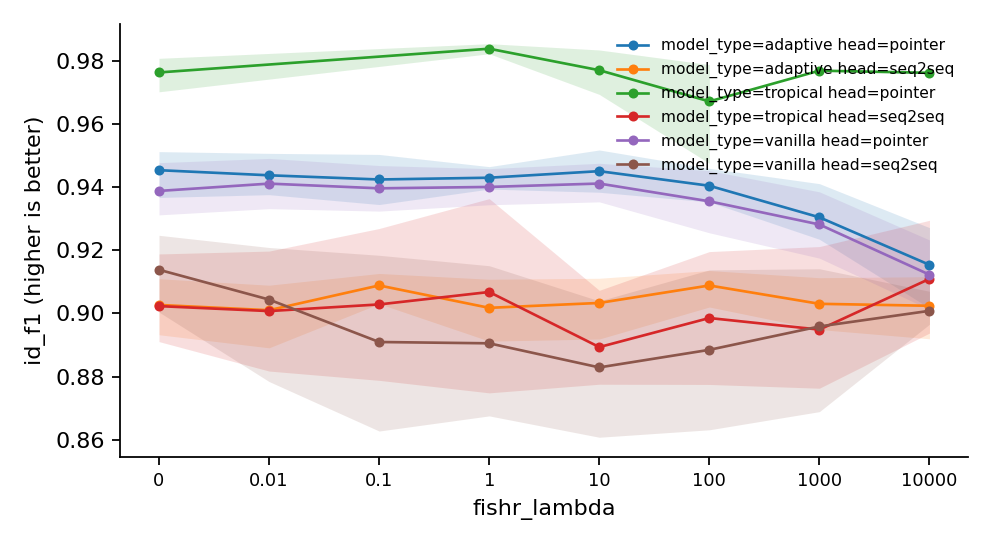
\includegraphics[width=\textwidth]{metric_id_f1.png}
\caption{\texttt{id\_f1} against \texttt{fishr\_lambda}: the mean over seeds with a 95\% bootstrap CI, one line per combination of the other factors.}
\label{fig:id_f1}
\end{figure}

{\small
\begin{longtable}{lllrlrrr}
\caption{\texttt{id\_f1} per cell: mean, 95\% bootstrap CI, SD, seeds, diverged runs.}\label{tab:summary-id_f1}\\
\toprule
\texttt{model\_type} & \texttt{head} & \texttt{fishr\_lambda} & mean & 95\% CI & SD & $n$ & div.\\
\midrule
\endhead
adaptive & pointer & 0 & 0.9453 & [0.937, 0.951] & 0.00983 & 5 & 0\\
adaptive & pointer & 0.01 & 0.9437 & [0.938, 0.951] & 0.0083 & 5 & 0\\
adaptive & pointer & 0.1 & 0.9424 & [0.934, 0.95] & 0.0101 & 5 & 0\\
adaptive & pointer & 1 & 0.9429 & [0.939, 0.946] & 0.00466 & 5 & 0\\
adaptive & pointer & 10 & 0.945 & [0.938, 0.952] & 0.00867 & 5 & 0\\
adaptive & pointer & 100 & 0.9404 & [0.935, 0.946] & 0.00728 & 5 & 0\\
adaptive & pointer & 1000 & 0.9304 & [0.923, 0.941] & 0.012 & 5 & 0\\
adaptive & pointer & 1e+04 & 0.9154 & [0.902, 0.927] & 0.0164 & 5 & 0\\
adaptive & seq2seq & 0 & 0.9027 & [0.893, 0.911] & 0.0119 & 5 & 0\\
adaptive & seq2seq & 0.01 & 0.901 & [0.889, 0.909] & 0.0134 & 5 & 0\\
adaptive & seq2seq & 0.1 & 0.9089 & [0.903, 0.913] & 0.00681 & 5 & 0\\
adaptive & seq2seq & 1 & 0.9018 & [0.891, 0.911] & 0.0128 & 5 & 0\\
adaptive & seq2seq & 10 & 0.9033 & [0.892, 0.911] & 0.0126 & 5 & 0\\
adaptive & seq2seq & 100 & 0.9088 & [0.902, 0.914] & 0.00769 & 5 & 0\\
adaptive & seq2seq & 1000 & 0.903 & [0.895, 0.911] & 0.0102 & 5 & 0\\
adaptive & seq2seq & 1e+04 & 0.9024 & [0.892, 0.912] & 0.0124 & 5 & 0\\
tropical & pointer & 0 & 0.9762 & [0.97, 0.981] & 0.00643 & 4 & 0\\
tropical & pointer & 1 & 0.9837 & [0.982, 0.985] & 0.00225 & 2 & 0\\
tropical & pointer & 10 & 0.9769 & [0.969, 0.983] & 0.0088 & 5 & 0\\
tropical & pointer & 100 & 0.9671 & [0.947, 0.979] & 0.0171 & 3 & 0\\
tropical & pointer & 1000 & 0.9768 & [--, --] & -- & 1 & 0\\
tropical & pointer & 1e+04 & 0.9761 & [--, --] & -- & 1 & 0\\
tropical & seq2seq & 0 & 0.9023 & [0.891, 0.919] & 0.0192 & 5 & 0\\
tropical & seq2seq & 0.01 & 0.9008 & [0.882, 0.92] & 0.0242 & 5 & 0\\
tropical & seq2seq & 0.1 & 0.9029 & [0.879, 0.927] & 0.031 & 5 & 0\\
tropical & seq2seq & 1 & 0.9068 & [0.875, 0.936] & 0.0404 & 5 & 0\\
tropical & seq2seq & 10 & 0.8894 & [0.878, 0.907] & 0.0199 & 5 & 0\\
tropical & seq2seq & 100 & 0.8986 & [0.878, 0.92] & 0.0276 & 5 & 0\\
tropical & seq2seq & 1000 & 0.8949 & [0.876, 0.921] & 0.0296 & 5 & 0\\
tropical & seq2seq & 1e+04 & 0.9109 & [0.894, 0.929] & 0.0232 & 5 & 0\\
vanilla & pointer & 0 & 0.9387 & [0.931, 0.948] & 0.0105 & 5 & 0\\
vanilla & pointer & 0.01 & 0.9411 & [0.933, 0.949] & 0.0103 & 5 & 0\\
vanilla & pointer & 0.1 & 0.9396 & [0.932, 0.947] & 0.00979 & 5 & 0\\
vanilla & pointer & 1 & 0.94 & [0.934, 0.946] & 0.00703 & 5 & 0\\
vanilla & pointer & 10 & 0.9411 & [0.935, 0.947] & 0.00826 & 5 & 0\\
vanilla & pointer & 100 & 0.9355 & [0.926, 0.945] & 0.0132 & 5 & 0\\
vanilla & pointer & 1000 & 0.9281 & [0.917, 0.938] & 0.0137 & 5 & 0\\
vanilla & pointer & 1e+04 & 0.9123 & [0.901, 0.923] & 0.0142 & 5 & 0\\
vanilla & seq2seq & 0 & 0.9138 & [0.9, 0.925] & 0.0152 & 5 & 0\\
vanilla & seq2seq & 0.01 & 0.9044 & [0.878, 0.921] & 0.0283 & 5 & 0\\
vanilla & seq2seq & 0.1 & 0.891 & [0.863, 0.918] & 0.0359 & 5 & 0\\
vanilla & seq2seq & 1 & 0.8906 & [0.868, 0.915] & 0.0304 & 5 & 0\\
vanilla & seq2seq & 10 & 0.8829 & [0.861, 0.904] & 0.0279 & 5 & 0\\
vanilla & seq2seq & 100 & 0.8885 & [0.863, 0.914] & 0.0336 & 5 & 0\\
vanilla & seq2seq & 1000 & 0.8959 & [0.869, 0.914] & 0.0299 & 5 & 0\\
vanilla & seq2seq & 1e+04 & 0.9008 & [0.897, 0.907] & 0.00671 & 5 & 0\\
\bottomrule
\end{longtable}
}

{\small
\begin{longtable}{lllrrrl}
\caption{\texttt{id\_f1}: each level of \texttt{fishr\_lambda} against its control (0), within each combination of the other factors. parametric: Dunnett vs control.}\label{tab:control-id_f1}\\
\toprule
\texttt{model\_type} & \texttt{head} & \texttt{fishr\_lambda} & difference & 95\% CI & $p$ & \\
\midrule
\endhead
adaptive & pointer & 0.01 & -0.001613 & [-0.0194, 0.0162] & 0.9999 & \\
adaptive & pointer & 0.1 & -0.002938 & [-0.0207, 0.0149] & 0.9973 & \\
adaptive & pointer & 1 & -0.00238 & [-0.0202, 0.0154] & 0.9993 & \\
adaptive & pointer & 10 & $-3.056\times10^{-4}$ & [-0.0181, 0.0175] & 1.0000 & \\
adaptive & pointer & 100 & -0.004921 & [-0.0227, 0.0129] & 0.9545 & \\
adaptive & pointer & 1000 & -0.01491 & [-0.0327, 0.0029] & 0.1314 & \\
adaptive & pointer & 1e+04 & -0.02993 & [-0.0477, -0.0121] & 0.0004 & *\\
adaptive & seq2seq & 0.01 & -0.001664 & [-0.0213, 0.018] & 1.0000 & \\
adaptive & seq2seq & 0.1 & 0.00617 & [-0.0134, 0.0258] & 0.9179 & \\
adaptive & seq2seq & 1 & $-9.163\times10^{-4}$ & [-0.0205, 0.0187] & 1.0000 & \\
adaptive & seq2seq & 10 & $6.308\times10^{-4}$ & [-0.019, 0.0202] & 1.0000 & \\
adaptive & seq2seq & 100 & 0.00616 & [-0.0135, 0.0258] & 0.9184 & \\
adaptive & seq2seq & 1000 & $3.563\times10^{-4}$ & [-0.0193, 0.02] & 1.0000 & \\
adaptive & seq2seq & 1e+04 & $-2.609\times10^{-4}$ & [-0.0199, 0.0194] & 1.0000 & \\
tropical & seq2seq & 0.01 & -0.001567 & [-0.0499, 0.0467] & 1.0000 & \\
tropical & seq2seq & 0.1 & $5.344\times10^{-4}$ & [-0.0478, 0.0488] & 1.0000 & \\
tropical & seq2seq & 1 & 0.004469 & [-0.0438, 0.0528] & 0.9999 & \\
tropical & seq2seq & 10 & -0.01296 & [-0.0613, 0.0354] & 0.9606 & \\
tropical & seq2seq & 100 & -0.003765 & [-0.0521, 0.0445] & 1.0000 & \\
tropical & seq2seq & 1000 & -0.007428 & [-0.0557, 0.0409] & 0.9983 & \\
tropical & seq2seq & 1e+04 & 0.008619 & [-0.0397, 0.0569] & 0.9957 & \\
vanilla & pointer & 0.01 & 0.002317 & [-0.0172, 0.0218] & 0.9997 & \\
vanilla & pointer & 0.1 & $8.281\times10^{-4}$ & [-0.0187, 0.0203] & 1.0000 & \\
vanilla & pointer & 1 & 0.001264 & [-0.0182, 0.0207] & 1.0000 & \\
vanilla & pointer & 10 & 0.00234 & [-0.0171, 0.0218] & 0.9996 & \\
vanilla & pointer & 100 & -0.003279 & [-0.0228, 0.0162] & 0.9970 & \\
vanilla & pointer & 1000 & -0.01061 & [-0.0301, 0.00887] & 0.5150 & \\
vanilla & pointer & 1e+04 & -0.02649 & [-0.046, -0.00701] & 0.0042 & *\\
vanilla & seq2seq & 0.01 & -0.009427 & [-0.0576, 0.0388] & 0.9927 & \\
vanilla & seq2seq & 0.1 & -0.02285 & [-0.0711, 0.0254] & 0.6523 & \\
vanilla & seq2seq & 1 & -0.02326 & [-0.0715, 0.0249] & 0.6353 & \\
vanilla & seq2seq & 10 & -0.03089 & [-0.0791, 0.0173] & 0.3499 & \\
vanilla & seq2seq & 100 & -0.02533 & [-0.0735, 0.0229] & 0.5517 & \\
vanilla & seq2seq & 1000 & -0.01793 & [-0.0661, 0.0303] & 0.8390 & \\
vanilla & seq2seq & 1e+04 & -0.01299 & [-0.0612, 0.0352] & 0.9598 & \\
\bottomrule
\end{longtable}
}

{\small
\begin{longtable}{llrrrrr}
\caption{\texttt{id\_f1} against log10 \texttt{fishr\_lambda}: parametric: OLS slope t-test, seed-bootstrap CI, with the Jonckheere--Terpstra ordered-trend $\tau$ and $p$.}\label{tab:trend-id_f1}\\
\toprule
\texttt{model\_type} & \texttt{head} & estimate & 95\% CI & $p$ & JT $\tau$ & JT $p$\\
\midrule
\endhead
adaptive & pointer & -0.003979 & [-0.00497, -0.00299] & 0.0002 & -0.459 & 0.0006\\
adaptive & seq2seq & $-1.220\times10^{-5}$ & [$-5.09\times10^{-4}$, $5.16\times10^{-4}$] & 0.9893 & -0.00571 & 0.9762\\
tropical & pointer & -0.0025 & [-0.00998, $-5.32\times10^{-4}$] & 0.3907 & -0.577 & 0.0382\\
tropical & seq2seq & $2.286\times10^{-4}$ & [-0.00336, 0.00279] & 0.9216 & 0.0514 & 0.7011\\
vanilla & pointer & -0.004066 & [-0.00548, -0.00219] & 0.0003 & -0.41 & 0.0032\\
vanilla & seq2seq & $-1.037\times10^{-4}$ & [-0.0027, 0.0025] & 0.9648 & -0.0857 & 0.5235\\
\bottomrule
\end{longtable}
}

{\small
\begin{longtable}{lrrrl}
\caption{\texttt{id\_f1}: paired contrasts by seed, Holm-corrected across the cells. parametric: paired t-test by seed, Holm.}\label{tab:paired-id_f1}\\
\toprule
contrast (within) & difference & 95\% CI & $p$ & \\
\midrule
\endhead
\stackcell{model\_type: tropical - vanilla\\\footnotesize head=pointer fishr\_lambda=0 } & 0.0343 & [0.0099, 0.0587] & 0.2289 & \\
\stackcell{model\_type: tropical - vanilla\\\footnotesize head=pointer fishr\_lambda=1 } & 0.04843 & [0.00212, 0.0947] & 0.4620 & \\
\stackcell{model\_type: tropical - vanilla\\\footnotesize head=pointer fishr\_lambda=10 } & 0.03585 & [0.0224, 0.0493] & 0.0216 & *\\
\stackcell{model\_type: tropical - vanilla\\\footnotesize head=pointer fishr\_lambda=100 } & 0.02583 & [0.00108, 0.0506] & 0.4620 & \\
\stackcell{model\_type: tropical - vanilla\\\footnotesize head=seq2seq fishr\_lambda=0 } & -0.0115 & [-0.0367, 0.0138] & 1.0000 & \\
\stackcell{model\_type: tropical - vanilla\\\footnotesize head=seq2seq fishr\_lambda=0.01 } & -0.00364 & [-0.0611, 0.0538] & 1.0000 & \\
\stackcell{model\_type: tropical - vanilla\\\footnotesize head=seq2seq fishr\_lambda=0.1 } & 0.01189 & [-0.0525, 0.0763] & 1.0000 & \\
\stackcell{model\_type: tropical - vanilla\\\footnotesize head=seq2seq fishr\_lambda=1 } & 0.01623 & [-0.0493, 0.0818] & 1.0000 & \\
\stackcell{model\_type: tropical - vanilla\\\footnotesize head=seq2seq fishr\_lambda=10 } & 0.006428 & [-0.0475, 0.0603] & 1.0000 & \\
\stackcell{model\_type: tropical - vanilla\\\footnotesize head=seq2seq fishr\_lambda=100 } & 0.01006 & [-0.0513, 0.0714] & 1.0000 & \\
\stackcell{model\_type: tropical - vanilla\\\footnotesize head=seq2seq fishr\_lambda=1000 } & $-9.976\times10^{-4}$ & [-0.0744, 0.0724] & 1.0000 & \\
\stackcell{model\_type: tropical - vanilla\\\footnotesize head=seq2seq fishr\_lambda=1e+04 } & 0.01011 & [-0.0212, 0.0414] & 1.0000 & \\
\stackcell{model\_type: adaptive - vanilla\\\footnotesize head=pointer fishr\_lambda=0 } & 0.006562 & [-0.0112, 0.0243] & 1.0000 & \\
\stackcell{model\_type: adaptive - vanilla\\\footnotesize head=pointer fishr\_lambda=0.01 } & 0.002633 & [-0.0104, 0.0156] & 1.0000 & \\
\stackcell{model\_type: adaptive - vanilla\\\footnotesize head=pointer fishr\_lambda=0.1 } & 0.002797 & [-0.00739, 0.013] & 1.0000 & \\
\stackcell{model\_type: adaptive - vanilla\\\footnotesize head=pointer fishr\_lambda=1 } & 0.002918 & [-0.00208, 0.00792] & 1.0000 & \\
\stackcell{model\_type: adaptive - vanilla\\\footnotesize head=pointer fishr\_lambda=10 } & 0.003916 & [-0.0112, 0.019] & 1.0000 & \\
\stackcell{model\_type: adaptive - vanilla\\\footnotesize head=pointer fishr\_lambda=100 } & 0.004921 & [-0.00454, 0.0144] & 1.0000 & \\
\stackcell{model\_type: adaptive - vanilla\\\footnotesize head=pointer fishr\_lambda=1000 } & 0.002269 & [-0.0282, 0.0327] & 1.0000 & \\
\stackcell{model\_type: adaptive - vanilla\\\footnotesize head=pointer fishr\_lambda=1e+04 } & 0.003122 & [-0.0213, 0.0276] & 1.0000 & \\
\stackcell{model\_type: adaptive - vanilla\\\footnotesize head=seq2seq fishr\_lambda=0 } & -0.01113 & [-0.0267, 0.00448] & 1.0000 & \\
\stackcell{model\_type: adaptive - vanilla\\\footnotesize head=seq2seq fishr\_lambda=0.01 } & -0.003365 & [-0.0473, 0.0406] & 1.0000 & \\
\stackcell{model\_type: adaptive - vanilla\\\footnotesize head=seq2seq fishr\_lambda=0.1 } & 0.01789 & [-0.0216, 0.0574] & 1.0000 & \\
\stackcell{model\_type: adaptive - vanilla\\\footnotesize head=seq2seq fishr\_lambda=1 } & 0.01122 & [-0.0192, 0.0416] & 1.0000 & \\
\stackcell{model\_type: adaptive - vanilla\\\footnotesize head=seq2seq fishr\_lambda=10 } & 0.02039 & [-0.0141, 0.0549] & 1.0000 & \\
\stackcell{model\_type: adaptive - vanilla\\\footnotesize head=seq2seq fishr\_lambda=100 } & 0.02036 & [-0.0177, 0.0584] & 1.0000 & \\
\stackcell{model\_type: adaptive - vanilla\\\footnotesize head=seq2seq fishr\_lambda=1000 } & 0.007158 & [-0.0232, 0.0375] & 1.0000 & \\
\stackcell{model\_type: adaptive - vanilla\\\footnotesize head=seq2seq fishr\_lambda=1e+04 } & 0.001599 & [-0.0141, 0.0173] & 1.0000 & \\
\stackcell{head: pointer - seq2seq\\\footnotesize model\_type=adaptive fishr\_lambda=0 } & 0.04262 & [0.0191, 0.0661] & 0.0883 & \\
\stackcell{head: pointer - seq2seq\\\footnotesize model\_type=adaptive fishr\_lambda=0.01 } & 0.04267 & [0.0271, 0.0583] & 0.0275 & *\\
\stackcell{head: pointer - seq2seq\\\footnotesize model\_type=adaptive fishr\_lambda=0.1 } & 0.03351 & [0.0188, 0.0482] & 0.0481 & *\\
\stackcell{head: pointer - seq2seq\\\footnotesize model\_type=adaptive fishr\_lambda=1 } & 0.04116 & [0.0263, 0.056] & 0.0275 & *\\
\stackcell{head: pointer - seq2seq\\\footnotesize model\_type=adaptive fishr\_lambda=10 } & 0.04168 & [0.0269, 0.0565] & 0.0273 & *\\
\stackcell{head: pointer - seq2seq\\\footnotesize model\_type=adaptive fishr\_lambda=100 } & 0.03154 & [0.0223, 0.0408] & 0.0137 & *\\
\stackcell{head: pointer - seq2seq\\\footnotesize model\_type=adaptive fishr\_lambda=1000 } & 0.02736 & [$2.34\times10^{-4}$, 0.0545] & 0.3187 & \\
\stackcell{head: pointer - seq2seq\\\footnotesize model\_type=adaptive fishr\_lambda=1e+04 } & 0.01295 & [0.00252, 0.0234] & 0.2613 & \\
\stackcell{head: pointer - seq2seq\\\footnotesize model\_type=tropical fishr\_lambda=0 } & 0.07169 & [0.0376, 0.106] & 0.0883 & \\
\stackcell{head: pointer - seq2seq\\\footnotesize model\_type=tropical fishr\_lambda=1 } & 0.1193 & [-0.0324, 0.271] & 0.3187 & \\
\stackcell{head: pointer - seq2seq\\\footnotesize model\_type=tropical fishr\_lambda=10 } & 0.08757 & [0.0522, 0.123] & 0.0374 & *\\
\stackcell{head: pointer - seq2seq\\\footnotesize model\_type=tropical fishr\_lambda=100 } & 0.07297 & [-0.0244, 0.17] & 0.3187 & \\
\stackcell{head: pointer - seq2seq\\\footnotesize model\_type=vanilla fishr\_lambda=0 } & 0.02493 & [0.0137, 0.0362] & 0.0494 & *\\
\stackcell{head: pointer - seq2seq\\\footnotesize model\_type=vanilla fishr\_lambda=0.01 } & 0.03667 & [-0.00519, 0.0785] & 0.3187 & \\
\stackcell{head: pointer - seq2seq\\\footnotesize model\_type=vanilla fishr\_lambda=0.1 } & 0.04861 & [0.00225, 0.095] & 0.3187 & \\
\stackcell{head: pointer - seq2seq\\\footnotesize model\_type=vanilla fishr\_lambda=1 } & 0.04946 & [0.00934, 0.0896] & 0.2613 & \\
\stackcell{head: pointer - seq2seq\\\footnotesize model\_type=vanilla fishr\_lambda=10 } & 0.05816 & [0.0186, 0.0977] & 0.1656 & \\
\stackcell{head: pointer - seq2seq\\\footnotesize model\_type=vanilla fishr\_lambda=100 } & 0.04698 & [0.00354, 0.0904] & 0.3187 & \\
\stackcell{head: pointer - seq2seq\\\footnotesize model\_type=vanilla fishr\_lambda=1000 } & 0.03225 & [0.00161, 0.0629] & 0.3187 & \\
\stackcell{head: pointer - seq2seq\\\footnotesize model\_type=vanilla fishr\_lambda=1e+04 } & 0.01143 & [-0.0113, 0.0341] & 0.3187 & \\
\bottomrule
\end{longtable}
}

\subsection{\texttt{id\_exact}}
\begin{figure}[tbp]
\centering
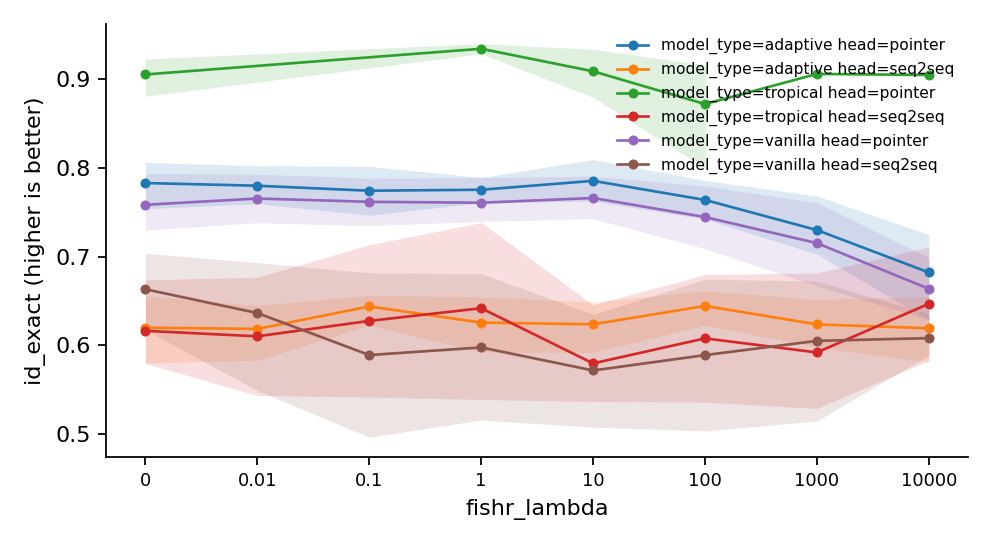
\includegraphics[width=\textwidth]{metric_id_exact.png}
\caption{\texttt{id\_exact} against \texttt{fishr\_lambda}: the mean over seeds with a 95\% bootstrap CI, one line per combination of the other factors.}
\label{fig:id_exact}
\end{figure}

{\small
\begin{longtable}{lllrlrrr}
\caption{\texttt{id\_exact} per cell: mean, 95\% bootstrap CI, SD, seeds, diverged runs.}\label{tab:summary-id_exact}\\
\toprule
\texttt{model\_type} & \texttt{head} & \texttt{fishr\_lambda} & mean & 95\% CI & SD & $n$ & div.\\
\midrule
\endhead
adaptive & pointer & 0 & 0.783 & [0.754, 0.806] & 0.0344 & 5 & 0\\
adaptive & pointer & 0.01 & 0.7799 & [0.76, 0.803] & 0.027 & 5 & 0\\
adaptive & pointer & 0.1 & 0.7743 & [0.747, 0.802] & 0.0364 & 5 & 0\\
adaptive & pointer & 1 & 0.7754 & [0.761, 0.789] & 0.018 & 5 & 0\\
adaptive & pointer & 10 & 0.7854 & [0.763, 0.809] & 0.0302 & 5 & 0\\
adaptive & pointer & 100 & 0.7639 & [0.742, 0.786] & 0.0302 & 5 & 0\\
adaptive & pointer & 1000 & 0.73 & [0.703, 0.768] & 0.0446 & 5 & 0\\
adaptive & pointer & 1e+04 & 0.6822 & [0.629, 0.725] & 0.0619 & 5 & 0\\
adaptive & seq2seq & 0 & 0.62 & [0.58, 0.656] & 0.0488 & 5 & 0\\
adaptive & seq2seq & 0.01 & 0.6186 & [0.583, 0.645] & 0.041 & 5 & 0\\
adaptive & seq2seq & 0.1 & 0.6439 & [0.623, 0.656] & 0.0235 & 5 & 0\\
adaptive & seq2seq & 1 & 0.6257 & [0.592, 0.655] & 0.0402 & 5 & 0\\
adaptive & seq2seq & 10 & 0.6238 & [0.592, 0.649] & 0.0382 & 5 & 0\\
adaptive & seq2seq & 100 & 0.6445 & [0.623, 0.661] & 0.025 & 5 & 0\\
adaptive & seq2seq & 1000 & 0.6237 & [0.598, 0.652] & 0.0338 & 5 & 0\\
adaptive & seq2seq & 1e+04 & 0.6193 & [0.581, 0.655] & 0.0471 & 5 & 0\\
tropical & pointer & 0 & 0.9053 & [0.881, 0.923] & 0.0259 & 4 & 0\\
tropical & pointer & 1 & 0.9343 & [0.929, 0.94] & 0.00806 & 2 & 0\\
tropical & pointer & 10 & 0.9089 & [0.88, 0.934] & 0.0331 & 5 & 0\\
tropical & pointer & 100 & 0.872 & [0.8, 0.916] & 0.0631 & 3 & 0\\
tropical & pointer & 1000 & 0.9059 & [--, --] & -- & 1 & 0\\
tropical & pointer & 1e+04 & 0.9047 & [--, --] & -- & 1 & 0\\
tropical & seq2seq & 0 & 0.6164 & [0.58, 0.674] & 0.0651 & 5 & 0\\
tropical & seq2seq & 0.01 & 0.6103 & [0.544, 0.677] & 0.0858 & 5 & 0\\
tropical & seq2seq & 0.1 & 0.6276 & [0.542, 0.713] & 0.11 & 5 & 0\\
tropical & seq2seq & 1 & 0.6419 & [0.539, 0.738] & 0.132 & 5 & 0\\
tropical & seq2seq & 10 & 0.5797 & [0.537, 0.646] & 0.0718 & 5 & 0\\
tropical & seq2seq & 100 & 0.6079 & [0.536, 0.68] & 0.0933 & 5 & 0\\
tropical & seq2seq & 1000 & 0.592 & [0.529, 0.682] & 0.102 & 5 & 0\\
tropical & seq2seq & 1e+04 & 0.6469 & [0.583, 0.711] & 0.0849 & 5 & 0\\
vanilla & pointer & 0 & 0.7585 & [0.73, 0.793] & 0.0407 & 5 & 0\\
vanilla & pointer & 0.01 & 0.7655 & [0.738, 0.793] & 0.035 & 5 & 0\\
vanilla & pointer & 0.1 & 0.7618 & [0.735, 0.789] & 0.0356 & 5 & 0\\
vanilla & pointer & 1 & 0.7608 & [0.74, 0.789] & 0.0315 & 5 & 0\\
vanilla & pointer & 10 & 0.7661 & [0.743, 0.791] & 0.0327 & 5 & 0\\
vanilla & pointer & 100 & 0.7446 & [0.709, 0.78] & 0.048 & 5 & 0\\
vanilla & pointer & 1000 & 0.7152 & [0.667, 0.761] & 0.0623 & 5 & 0\\
vanilla & pointer & 1e+04 & 0.6638 & [0.629, 0.699] & 0.046 & 5 & 0\\
vanilla & seq2seq & 0 & 0.6633 & [0.617, 0.704] & 0.0548 & 5 & 0\\
vanilla & seq2seq & 0.01 & 0.6365 & [0.549, 0.693] & 0.0955 & 5 & 0\\
vanilla & seq2seq & 0.1 & 0.5891 & [0.497, 0.682] & 0.119 & 5 & 0\\
vanilla & seq2seq & 1 & 0.5977 & [0.516, 0.681] & 0.107 & 5 & 0\\
vanilla & seq2seq & 10 & 0.5718 & [0.508, 0.635] & 0.0811 & 5 & 0\\
vanilla & seq2seq & 100 & 0.5891 & [0.504, 0.675] & 0.112 & 5 & 0\\
vanilla & seq2seq & 1000 & 0.6051 & [0.515, 0.673] & 0.104 & 5 & 0\\
vanilla & seq2seq & 1e+04 & 0.6082 & [0.589, 0.635] & 0.0307 & 5 & 0\\
\bottomrule
\end{longtable}
}

{\small
\begin{longtable}{lllrrrl}
\caption{\texttt{id\_exact}: each level of \texttt{fishr\_lambda} against its control (0), within each combination of the other factors. parametric: Dunnett vs control.}\label{tab:control-id_exact}\\
\toprule
\texttt{model\_type} & \texttt{head} & \texttt{fishr\_lambda} & difference & 95\% CI & $p$ & \\
\midrule
\endhead
adaptive & pointer & 0.01 & -0.00304 & [-0.0684, 0.0623] & 1.0000 & \\
adaptive & pointer & 0.1 & -0.00866 & [-0.074, 0.0567] & 0.9993 & \\
adaptive & pointer & 1 & -0.00756 & [-0.0729, 0.0578] & 0.9997 & \\
adaptive & pointer & 10 & 0.00248 & [-0.0629, 0.0678] & 1.0000 & \\
adaptive & pointer & 100 & -0.01902 & [-0.0844, 0.0463] & 0.9420 & \\
adaptive & pointer & 1000 & -0.05298 & [-0.118, 0.0124] & 0.1518 & \\
adaptive & pointer & 1e+04 & -0.1008 & [-0.166, -0.0354] & 0.0011 & *\\
adaptive & seq2seq & 0.01 & -0.00142 & [-0.0681, 0.0653] & 1.0000 & \\
adaptive & seq2seq & 0.1 & 0.02392 & [-0.0428, 0.0906] & 0.8599 & \\
adaptive & seq2seq & 1 & 0.0057 & [-0.061, 0.0724] & 1.0000 & \\
adaptive & seq2seq & 10 & 0.0038 & [-0.0629, 0.0705] & 1.0000 & \\
adaptive & seq2seq & 100 & 0.02448 & [-0.0422, 0.0912] & 0.8470 & \\
adaptive & seq2seq & 1000 & 0.0037 & [-0.063, 0.0704] & 1.0000 & \\
adaptive & seq2seq & 1e+04 & $-7.000\times10^{-4}$ & [-0.0674, 0.066] & 1.0000 & \\
tropical & seq2seq & 0.01 & -0.00616 & [-0.173, 0.16] & 1.0000 & \\
tropical & seq2seq & 0.1 & 0.01118 & [-0.155, 0.178] & 1.0000 & \\
tropical & seq2seq & 1 & 0.0255 & [-0.141, 0.192] & 0.9983 & \\
tropical & seq2seq & 10 & -0.0367 & [-0.203, 0.13] & 0.9858 & \\
tropical & seq2seq & 100 & -0.00848 & [-0.175, 0.158] & 1.0000 & \\
tropical & seq2seq & 1000 & -0.02438 & [-0.191, 0.142] & 0.9987 & \\
tropical & seq2seq & 1e+04 & 0.03052 & [-0.136, 0.197] & 0.9950 & \\
vanilla & pointer & 0.01 & 0.00706 & [-0.0674, 0.0815] & 0.9999 & \\
vanilla & pointer & 0.1 & 0.00334 & [-0.0711, 0.0778] & 1.0000 & \\
vanilla & pointer & 1 & 0.0023 & [-0.0721, 0.0767] & 1.0000 & \\
vanilla & pointer & 10 & 0.00764 & [-0.0668, 0.0821] & 0.9999 & \\
vanilla & pointer & 100 & -0.01382 & [-0.0882, 0.0606] & 0.9946 & \\
vanilla & pointer & 1000 & -0.04322 & [-0.118, 0.0312] & 0.4491 & \\
vanilla & pointer & 1e+04 & -0.09466 & [-0.169, -0.0202] & 0.0080 & *\\
vanilla & seq2seq & 0.01 & -0.0268 & [-0.189, 0.135] & 0.9973 & \\
vanilla & seq2seq & 0.1 & -0.07414 & [-0.236, 0.0877] & 0.6834 & \\
vanilla & seq2seq & 1 & -0.06556 & [-0.227, 0.0963] & 0.7830 & \\
vanilla & seq2seq & 10 & -0.0915 & [-0.253, 0.0703] & 0.4769 & \\
vanilla & seq2seq & 100 & -0.0742 & [-0.236, 0.0876] & 0.6825 & \\
vanilla & seq2seq & 1000 & -0.05814 & [-0.22, 0.104] & 0.8587 & \\
vanilla & seq2seq & 1e+04 & -0.05508 & [-0.217, 0.107] & 0.8858 & \\
\bottomrule
\end{longtable}
}

{\small
\begin{longtable}{llrrrrr}
\caption{\texttt{id\_exact} against log10 \texttt{fishr\_lambda}: parametric: OLS slope t-test, seed-bootstrap CI, with the Jonckheere--Terpstra ordered-trend $\tau$ and $p$.}\label{tab:trend-id_exact}\\
\toprule
\texttt{model\_type} & \texttt{head} & estimate & 95\% CI & $p$ & JT $\tau$ & JT $p$\\
\midrule
\endhead
adaptive & pointer & -0.01404 & [-0.0178, -0.0103] & 0.0003 & -0.446 & 0.0006\\
adaptive & seq2seq & $-6.964\times10^{-4}$ & [-0.00172, $4.16\times10^{-4}$] & 0.8160 & -0.0133 & 0.9268\\
tropical & pointer & -0.009767 & [-0.0371, -0.00226] & 0.3666 & -0.538 & 0.0510\\
tropical & seq2seq & $1.764\times10^{-4}$ & [-0.0141, 0.011] & 0.9825 & 0.0267 & 0.8484\\
vanilla & pointer & -0.0148 & [-0.0198, -0.0079] & 0.0004 & -0.402 & 0.0036\\
vanilla & seq2seq & -0.002196 & [-0.0113, 0.0069] & 0.7775 & -0.0552 & 0.6925\\
\bottomrule
\end{longtable}
}

{\small
\begin{longtable}{lrrrl}
\caption{\texttt{id\_exact}: paired contrasts by seed, Holm-corrected across the cells. parametric: paired t-test by seed, Holm.}\label{tab:paired-id_exact}\\
\toprule
contrast (within) & difference & 95\% CI & $p$ & \\
\midrule
\endhead
\stackcell{model\_type: tropical - vanilla\\\footnotesize head=pointer fishr\_lambda=0 } & 0.1347 & [0.0378, 0.232] & 0.2360 & \\
\stackcell{model\_type: tropical - vanilla\\\footnotesize head=pointer fishr\_lambda=1 } & 0.1933 & [0.0898, 0.297] & 0.2682 & \\
\stackcell{model\_type: tropical - vanilla\\\footnotesize head=pointer fishr\_lambda=10 } & 0.1428 & [0.0857, 0.2] & 0.0270 & *\\
\stackcell{model\_type: tropical - vanilla\\\footnotesize head=pointer fishr\_lambda=100 } & 0.1069 & [0.0149, 0.199] & 0.3402 & \\
\stackcell{model\_type: tropical - vanilla\\\footnotesize head=seq2seq fishr\_lambda=0 } & -0.04684 & [-0.139, 0.0451] & 1.0000 & \\
\stackcell{model\_type: tropical - vanilla\\\footnotesize head=seq2seq fishr\_lambda=0.01 } & -0.0262 & [-0.218, 0.165] & 1.0000 & \\
\stackcell{model\_type: tropical - vanilla\\\footnotesize head=seq2seq fishr\_lambda=0.1 } & 0.03848 & [-0.177, 0.254] & 1.0000 & \\
\stackcell{model\_type: tropical - vanilla\\\footnotesize head=seq2seq fishr\_lambda=1 } & 0.04422 & [-0.179, 0.267] & 1.0000 & \\
\stackcell{model\_type: tropical - vanilla\\\footnotesize head=seq2seq fishr\_lambda=10 } & 0.00796 & [-0.158, 0.174] & 1.0000 & \\
\stackcell{model\_type: tropical - vanilla\\\footnotesize head=seq2seq fishr\_lambda=100 } & 0.01888 & [-0.184, 0.222] & 1.0000 & \\
\stackcell{model\_type: tropical - vanilla\\\footnotesize head=seq2seq fishr\_lambda=1000 } & -0.01308 & [-0.267, 0.241] & 1.0000 & \\
\stackcell{model\_type: tropical - vanilla\\\footnotesize head=seq2seq fishr\_lambda=1e+04 } & 0.03876 & [-0.0813, 0.159] & 1.0000 & \\
\stackcell{model\_type: adaptive - vanilla\\\footnotesize head=pointer fishr\_lambda=0 } & 0.0245 & [-0.0391, 0.0881] & 1.0000 & \\
\stackcell{model\_type: adaptive - vanilla\\\footnotesize head=pointer fishr\_lambda=0.01 } & 0.0144 & [-0.0286, 0.0574] & 1.0000 & \\
\stackcell{model\_type: adaptive - vanilla\\\footnotesize head=pointer fishr\_lambda=0.1 } & 0.0125 & [-0.0215, 0.0465] & 1.0000 & \\
\stackcell{model\_type: adaptive - vanilla\\\footnotesize head=pointer fishr\_lambda=1 } & 0.01464 & [-0.00856, 0.0378] & 1.0000 & \\
\stackcell{model\_type: adaptive - vanilla\\\footnotesize head=pointer fishr\_lambda=10 } & 0.01934 & [-0.0392, 0.0779] & 1.0000 & \\
\stackcell{model\_type: adaptive - vanilla\\\footnotesize head=pointer fishr\_lambda=100 } & 0.0193 & [-0.0123, 0.0509] & 1.0000 & \\
\stackcell{model\_type: adaptive - vanilla\\\footnotesize head=pointer fishr\_lambda=1000 } & 0.01474 & [-0.112, 0.142] & 1.0000 & \\
\stackcell{model\_type: adaptive - vanilla\\\footnotesize head=pointer fishr\_lambda=1e+04 } & 0.0184 & [-0.0728, 0.11] & 1.0000 & \\
\stackcell{model\_type: adaptive - vanilla\\\footnotesize head=seq2seq fishr\_lambda=0 } & -0.04326 & [-0.103, 0.0162] & 1.0000 & \\
\stackcell{model\_type: adaptive - vanilla\\\footnotesize head=seq2seq fishr\_lambda=0.01 } & -0.01788 & [-0.164, 0.128] & 1.0000 & \\
\stackcell{model\_type: adaptive - vanilla\\\footnotesize head=seq2seq fishr\_lambda=0.1 } & 0.0548 & [-0.0731, 0.183] & 1.0000 & \\
\stackcell{model\_type: adaptive - vanilla\\\footnotesize head=seq2seq fishr\_lambda=1 } & 0.028 & [-0.0788, 0.135] & 1.0000 & \\
\stackcell{model\_type: adaptive - vanilla\\\footnotesize head=seq2seq fishr\_lambda=10 } & 0.05204 & [-0.0582, 0.162] & 1.0000 & \\
\stackcell{model\_type: adaptive - vanilla\\\footnotesize head=seq2seq fishr\_lambda=100 } & 0.05542 & [-0.0734, 0.184] & 1.0000 & \\
\stackcell{model\_type: adaptive - vanilla\\\footnotesize head=seq2seq fishr\_lambda=1000 } & 0.01858 & [-0.0981, 0.135] & 1.0000 & \\
\stackcell{model\_type: adaptive - vanilla\\\footnotesize head=seq2seq fishr\_lambda=1e+04 } & 0.01112 & [-0.043, 0.0652] & 1.0000 & \\
\stackcell{head: pointer - seq2seq\\\footnotesize model\_type=adaptive fishr\_lambda=0 } & 0.163 & [0.0729, 0.253] & 0.0884 & \\
\stackcell{head: pointer - seq2seq\\\footnotesize model\_type=adaptive fishr\_lambda=0.01 } & 0.1613 & [0.114, 0.209] & 0.0128 & *\\
\stackcell{head: pointer - seq2seq\\\footnotesize model\_type=adaptive fishr\_lambda=0.1 } & 0.1304 & [0.0773, 0.183] & 0.0362 & *\\
\stackcell{head: pointer - seq2seq\\\footnotesize model\_type=adaptive fishr\_lambda=1 } & 0.1497 & [0.103, 0.197] & 0.0153 & *\\
\stackcell{head: pointer - seq2seq\\\footnotesize model\_type=adaptive fishr\_lambda=10 } & 0.1616 & [0.121, 0.202] & 0.0069 & *\\
\stackcell{head: pointer - seq2seq\\\footnotesize model\_type=adaptive fishr\_lambda=100 } & 0.1195 & [0.0903, 0.149] & 0.0069 & *\\
\stackcell{head: pointer - seq2seq\\\footnotesize model\_type=adaptive fishr\_lambda=1000 } & 0.1063 & [0.0121, 0.2] & 0.3159 & \\
\stackcell{head: pointer - seq2seq\\\footnotesize model\_type=adaptive fishr\_lambda=1e+04 } & 0.0629 & [0.0232, 0.103] & 0.1291 & \\
\stackcell{head: pointer - seq2seq\\\footnotesize model\_type=tropical fishr\_lambda=0 } & 0.2837 & [0.163, 0.404] & 0.0642 & \\
\stackcell{head: pointer - seq2seq\\\footnotesize model\_type=tropical fishr\_lambda=1 } & 0.4278 & [-0.145, 1] & 0.3159 & \\
\stackcell{head: pointer - seq2seq\\\footnotesize model\_type=tropical fishr\_lambda=10 } & 0.3291 & [0.2, 0.458] & 0.0339 & *\\
\stackcell{head: pointer - seq2seq\\\footnotesize model\_type=tropical fishr\_lambda=100 } & 0.279 & [-0.0412, 0.599] & 0.3159 & \\
\stackcell{head: pointer - seq2seq\\\footnotesize model\_type=vanilla fishr\_lambda=0 } & 0.0952 & [0.0533, 0.137] & 0.0451 & *\\
\stackcell{head: pointer - seq2seq\\\footnotesize model\_type=vanilla fishr\_lambda=0.01 } & 0.1291 & [-0.0133, 0.271] & 0.3159 & \\
\stackcell{head: pointer - seq2seq\\\footnotesize model\_type=vanilla fishr\_lambda=0.1 } & 0.1727 & [0.0177, 0.328] & 0.3159 & \\
\stackcell{head: pointer - seq2seq\\\footnotesize model\_type=vanilla fishr\_lambda=1 } & 0.1631 & [0.0122, 0.314] & 0.3159 & \\
\stackcell{head: pointer - seq2seq\\\footnotesize model\_type=vanilla fishr\_lambda=10 } & 0.1943 & [0.0684, 0.32] & 0.1291 & \\
\stackcell{head: pointer - seq2seq\\\footnotesize model\_type=vanilla fishr\_lambda=100 } & 0.1556 & [0.00979, 0.301] & 0.3159 & \\
\stackcell{head: pointer - seq2seq\\\footnotesize model\_type=vanilla fishr\_lambda=1000 } & 0.1101 & [-0.00663, 0.227] & 0.3159 & \\
\stackcell{head: pointer - seq2seq\\\footnotesize model\_type=vanilla fishr\_lambda=1e+04 } & 0.05562 & [-0.0227, 0.134] & 0.3159 & \\
\bottomrule
\end{longtable}
}


\section{Curves}
\begin{figure}[tbp]
\centering
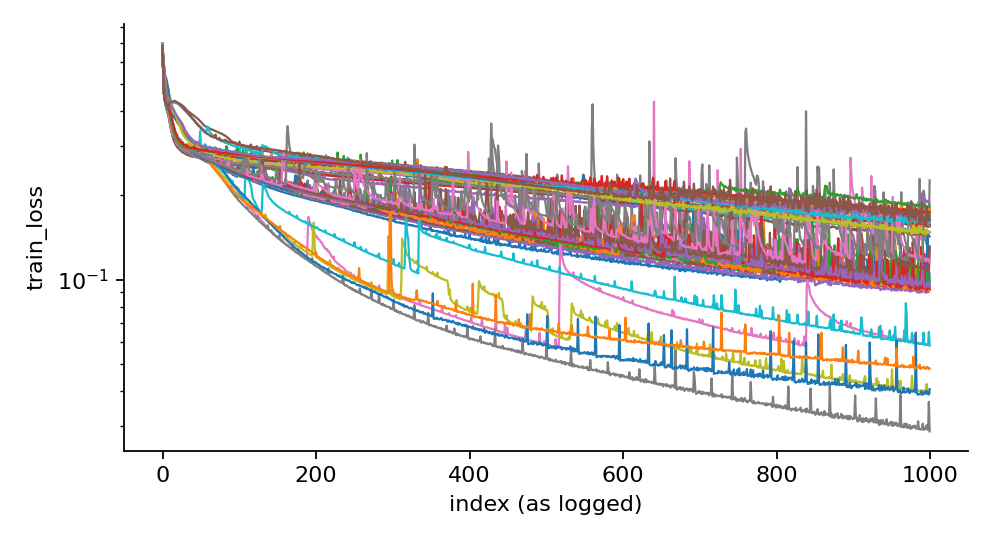
\includegraphics[width=\textwidth]{curve_train_loss.png}
\caption{\texttt{train\_loss}, the mean over seeds per cell.}
\label{fig:curve-1}
\end{figure}
\begin{figure}[tbp]
\centering
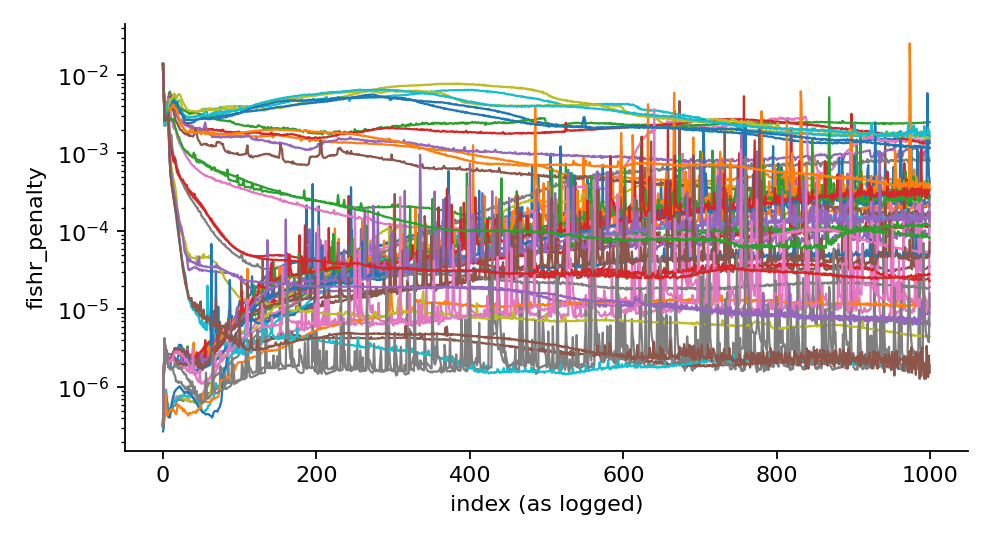
\includegraphics[width=\textwidth]{curve_fishr_penalty.png}
\caption{\texttt{fishr\_penalty}, the mean over seeds per cell.}
\label{fig:curve-2}
\end{figure}
\begin{figure}[tbp]
\centering
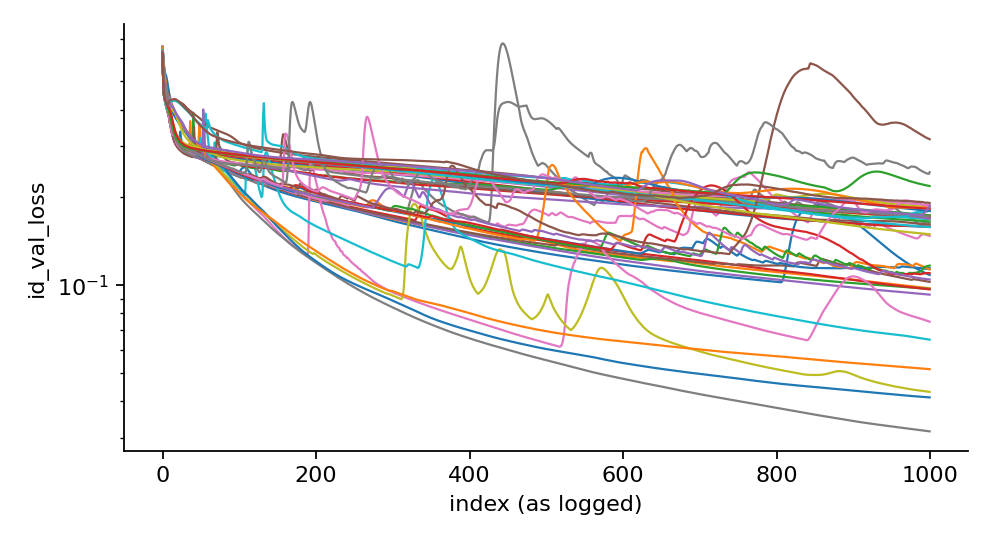
\includegraphics[width=\textwidth]{curve_id_val_loss.png}
\caption{\texttt{id\_val\_loss}, the mean over seeds per cell.}
\label{fig:curve-3}
\end{figure}

\section{Configuration}
The base configuration every run shares (frozen hash \texttt{2737a4a4d758}); factor levels are in \autoref{tab:summary-ood_len_f1}.
{\footnotesize
\begin{verbatim}
task:
  name: BinPackingDataset
  value_range:
  - 1
  - 10
  target_range:
  - 10
  - 30
  weight_range: null
  adversarial_range:
  - 10
  - 30
  noise_prob: 0.0
data:
  train_lengths:
  - 4
  - 5
  - 6
  - 7
  - 8
  ood_lengths:
  - 12
  - 16
  - 64
  ood_value_range:
  - 11
  - 100
  ood_noise_range:
  - 10
  - 30
  ood_noise_prob: 0.5
  n_per_length: 20000
  n_eval_per_length: 2000
  curve_eval_limit: 256
model:
  d_model: 64
  n_heads: 2
  num_layers: 1
  dropout: 0.0
  tropical_impl: legacy
optim:
  lr: 0.0001
  epochs: 1000
  batch_size: 100
  eval_batch_size: 256
fishr:
  ema: 0.95
  anneal_iters: 1500
  reset_optimizer: true
\end{verbatim}
}
Store: \texttt{campaigns/tropical/BinPacking/results}.
\end{document}